\documentclass[twoside]{book}

% Packages required by doxygen
\usepackage{fixltx2e}
\usepackage{calc}
\usepackage{doxygen}
\usepackage[export]{adjustbox} % also loads graphicx
\usepackage{graphicx}
\usepackage[utf8]{inputenc}
\usepackage{makeidx}
\usepackage{multicol}
\usepackage{multirow}
\PassOptionsToPackage{warn}{textcomp}
\usepackage{textcomp}
\usepackage[nointegrals]{wasysym}
\usepackage[table]{xcolor}

% Font selection
\usepackage[T1]{fontenc}
\usepackage[scaled=.90]{helvet}
\usepackage{courier}
\usepackage{amssymb}
\usepackage{sectsty}
\renewcommand{\familydefault}{\sfdefault}
\allsectionsfont{%
  \fontseries{bc}\selectfont%
  \color{darkgray}%
}
\renewcommand{\DoxyLabelFont}{%
  \fontseries{bc}\selectfont%
  \color{darkgray}%
}
\newcommand{\+}{\discretionary{\mbox{\scriptsize$\hookleftarrow$}}{}{}}

% Page & text layout
\usepackage{geometry}
\geometry{%
  a4paper,%
  top=2.5cm,%
  bottom=2.5cm,%
  left=2.5cm,%
  right=2.5cm%
}
\tolerance=750
\hfuzz=15pt
\hbadness=750
\setlength{\emergencystretch}{15pt}
\setlength{\parindent}{0cm}
\setlength{\parskip}{3ex plus 2ex minus 2ex}
\makeatletter
\renewcommand{\paragraph}{%
  \@startsection{paragraph}{4}{0ex}{-1.0ex}{1.0ex}{%
    \normalfont\normalsize\bfseries\SS@parafont%
  }%
}
\renewcommand{\subparagraph}{%
  \@startsection{subparagraph}{5}{0ex}{-1.0ex}{1.0ex}{%
    \normalfont\normalsize\bfseries\SS@subparafont%
  }%
}
\makeatother

% Headers & footers
\usepackage{fancyhdr}
\pagestyle{fancyplain}
\fancyhead[LE]{\fancyplain{}{\bfseries\thepage}}
\fancyhead[CE]{\fancyplain{}{}}
\fancyhead[RE]{\fancyplain{}{\bfseries\leftmark}}
\fancyhead[LO]{\fancyplain{}{\bfseries\rightmark}}
\fancyhead[CO]{\fancyplain{}{}}
\fancyhead[RO]{\fancyplain{}{\bfseries\thepage}}
\fancyfoot[LE]{\fancyplain{}{}}
\fancyfoot[CE]{\fancyplain{}{}}
\fancyfoot[RE]{\fancyplain{}{\bfseries\scriptsize Generated by Doxygen }}
\fancyfoot[LO]{\fancyplain{}{\bfseries\scriptsize Generated by Doxygen }}
\fancyfoot[CO]{\fancyplain{}{}}
\fancyfoot[RO]{\fancyplain{}{}}
\renewcommand{\footrulewidth}{0.4pt}
\renewcommand{\chaptermark}[1]{%
  \markboth{#1}{}%
}
\renewcommand{\sectionmark}[1]{%
  \markright{\thesection\ #1}%
}

% Indices & bibliography
\usepackage{natbib}
\usepackage[titles]{tocloft}
\setcounter{tocdepth}{3}
\setcounter{secnumdepth}{5}
\makeindex

% Hyperlinks (required, but should be loaded last)
\usepackage{ifpdf}
\ifpdf
  \usepackage[pdftex,pagebackref=true]{hyperref}
\else
  \usepackage[ps2pdf,pagebackref=true]{hyperref}
\fi
\hypersetup{%
  colorlinks=true,%
  linkcolor=blue,%
  citecolor=blue,%
  unicode%
}

% Custom commands
\newcommand{\clearemptydoublepage}{%
  \newpage{\pagestyle{empty}\cleardoublepage}%
}

\usepackage{caption}
\captionsetup{labelsep=space,justification=centering,font={bf},singlelinecheck=off,skip=4pt,position=top}

%===== C O N T E N T S =====

\begin{document}

% Titlepage & ToC
\hypersetup{pageanchor=false,
             bookmarksnumbered=true,
             pdfencoding=unicode
            }
\pagenumbering{alph}
\begin{titlepage}
\vspace*{7cm}
\begin{center}%
{\Large S\+O\+F\+T\+ON groep 9 }\\
\vspace*{1cm}
{\large Generated by Doxygen 1.8.13}\\
\end{center}
\end{titlepage}
\clearemptydoublepage
\pagenumbering{roman}
\tableofcontents
\clearemptydoublepage
\pagenumbering{arabic}
\hypersetup{pageanchor=true}

%--- Begin generated contents ---
\chapter{File Index}
\section{File List}
Here is a list of all files with brief descriptions\+:\begin{DoxyCompactList}
\item\contentsline{section}{\hyperlink{includes_8h}{includes.\+h} }{\pageref{includes_8h}}{}
\item\contentsline{section}{\hyperlink{main_8c}{main.\+c} }{\pageref{main_8c}}{}
\item\contentsline{section}{\hyperlink{main_8h}{main.\+h} }{\pageref{main_8h}}{}
\item\contentsline{section}{logic\+\_\+layer/\hyperlink{_draw__request_8c}{Draw\+\_\+request.\+c} }{\pageref{_draw__request_8c}}{}
\item\contentsline{section}{logic\+\_\+layer/\hyperlink{_draw__request_8h}{Draw\+\_\+request.\+h} }{\pageref{_draw__request_8h}}{}
\item\contentsline{section}{logic\+\_\+layer/\hyperlink{uitvoer_8h}{uitvoer.\+h} }{\pageref{uitvoer_8h}}{}
\item\contentsline{section}{Presentation\+\_\+layer/\hyperlink{presentation_8c}{presentation.\+c} }{\pageref{presentation_8c}}{}
\item\contentsline{section}{Presentation\+\_\+layer/\hyperlink{presentation_8h}{presentation.\+h} }{\pageref{presentation_8h}}{}
\end{DoxyCompactList}

\chapter{File Documentation}
\hypertarget{includes_8h}{}\section{includes.\+h File Reference}
\label{includes_8h}\index{includes.\+h@{includes.\+h}}
{\ttfamily \#include $<$stdarg.\+h$>$}\newline
{\ttfamily \#include $<$stdio.\+h$>$}\newline
{\ttfamily \#include $<$stdlib.\+h$>$}\newline
{\ttfamily \#include $<$math.\+h$>$}\newline
{\ttfamily \#include $<$string.\+h$>$}\newline
{\ttfamily \#include $<$bfc\+\_\+latin\+\_\+font.\+h$>$}\newline
{\ttfamily \#include \char`\"{}misc.\+h\char`\"{}}\newline
{\ttfamily \#include \char`\"{}stm32f4xx\+\_\+rcc.\+h\char`\"{}}\newline
{\ttfamily \#include \char`\"{}stm32f4xx\+\_\+gpio.\+h\char`\"{}}\newline
{\ttfamily \#include \char`\"{}stm32f4xx\+\_\+usart.\+h\char`\"{}}\newline
{\ttfamily \#include \char`\"{}stm32\+\_\+ub\+\_\+vga\+\_\+screen.\+h\char`\"{}}\newline
{\ttfamily \#include \char`\"{}uart.\+h\char`\"{}}\newline
{\ttfamily \#include \char`\"{}delay.\+h\char`\"{}}\newline
{\ttfamily \#include \char`\"{}Draw\+\_\+request.\+h\char`\"{}}\newline
{\ttfamily \#include \char`\"{}presentation.\+h\char`\"{}}\newline
Include dependency graph for includes.\+h\+:\nopagebreak
\begin{figure}[H]
\begin{center}
\leavevmode
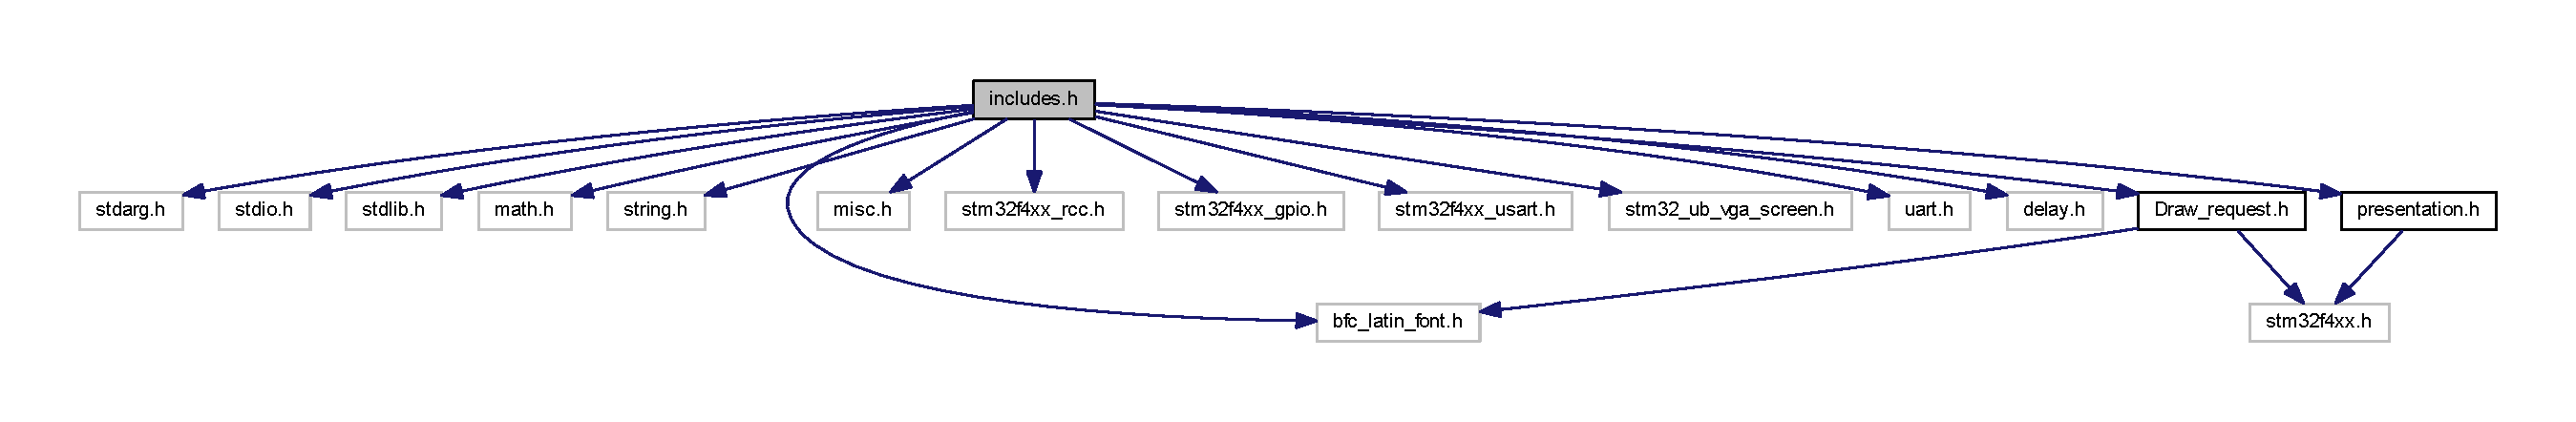
\includegraphics[width=350pt]{includes_8h__incl}
\end{center}
\end{figure}
This graph shows which files directly or indirectly include this file\+:\nopagebreak
\begin{figure}[H]
\begin{center}
\leavevmode
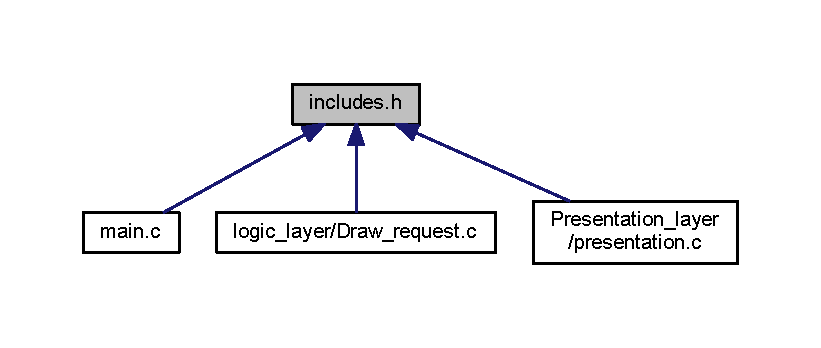
\includegraphics[width=350pt]{includes_8h__dep__incl}
\end{center}
\end{figure}
\subsection*{Macros}
\begin{DoxyCompactItemize}
\item 
\#define \hyperlink{includes_8h_af4bcb3fa5c2b8fe0b9f71e52f76abb28}{O\+S\+\_\+\+M\+A\+S\+T\+E\+R\+\_\+\+F\+I\+LE}
\item 
\#define \hyperlink{includes_8h_a706068f562dd5c64a8b7bbd4b2298dd1}{M\+A\+X\+\_\+\+L\+I\+N\+E\+\_\+\+S\+I\+ZE}~64
\item 
\#define \hyperlink{includes_8h_aa8cecfc5c5c054d2875c03e77b7be15d}{T\+R\+UE}~1
\item 
\#define \hyperlink{includes_8h_aa93f0eb578d23995850d61f7d61c55c1}{F\+A\+L\+SE}~0
\end{DoxyCompactItemize}


\subsection{Macro Definition Documentation}
\mbox{\Hypertarget{includes_8h_aa93f0eb578d23995850d61f7d61c55c1}\label{includes_8h_aa93f0eb578d23995850d61f7d61c55c1}} 
\index{includes.\+h@{includes.\+h}!F\+A\+L\+SE@{F\+A\+L\+SE}}
\index{F\+A\+L\+SE@{F\+A\+L\+SE}!includes.\+h@{includes.\+h}}
\subsubsection{\texorpdfstring{F\+A\+L\+SE}{FALSE}}
{\footnotesize\ttfamily \#define F\+A\+L\+SE~0}

\mbox{\Hypertarget{includes_8h_a706068f562dd5c64a8b7bbd4b2298dd1}\label{includes_8h_a706068f562dd5c64a8b7bbd4b2298dd1}} 
\index{includes.\+h@{includes.\+h}!M\+A\+X\+\_\+\+L\+I\+N\+E\+\_\+\+S\+I\+ZE@{M\+A\+X\+\_\+\+L\+I\+N\+E\+\_\+\+S\+I\+ZE}}
\index{M\+A\+X\+\_\+\+L\+I\+N\+E\+\_\+\+S\+I\+ZE@{M\+A\+X\+\_\+\+L\+I\+N\+E\+\_\+\+S\+I\+ZE}!includes.\+h@{includes.\+h}}
\subsubsection{\texorpdfstring{M\+A\+X\+\_\+\+L\+I\+N\+E\+\_\+\+S\+I\+ZE}{MAX\_LINE\_SIZE}}
{\footnotesize\ttfamily \#define M\+A\+X\+\_\+\+L\+I\+N\+E\+\_\+\+S\+I\+ZE~64}

\mbox{\Hypertarget{includes_8h_af4bcb3fa5c2b8fe0b9f71e52f76abb28}\label{includes_8h_af4bcb3fa5c2b8fe0b9f71e52f76abb28}} 
\index{includes.\+h@{includes.\+h}!O\+S\+\_\+\+M\+A\+S\+T\+E\+R\+\_\+\+F\+I\+LE@{O\+S\+\_\+\+M\+A\+S\+T\+E\+R\+\_\+\+F\+I\+LE}}
\index{O\+S\+\_\+\+M\+A\+S\+T\+E\+R\+\_\+\+F\+I\+LE@{O\+S\+\_\+\+M\+A\+S\+T\+E\+R\+\_\+\+F\+I\+LE}!includes.\+h@{includes.\+h}}
\subsubsection{\texorpdfstring{O\+S\+\_\+\+M\+A\+S\+T\+E\+R\+\_\+\+F\+I\+LE}{OS\_MASTER\_FILE}}
{\footnotesize\ttfamily \#define O\+S\+\_\+\+M\+A\+S\+T\+E\+R\+\_\+\+F\+I\+LE}

\mbox{\Hypertarget{includes_8h_aa8cecfc5c5c054d2875c03e77b7be15d}\label{includes_8h_aa8cecfc5c5c054d2875c03e77b7be15d}} 
\index{includes.\+h@{includes.\+h}!T\+R\+UE@{T\+R\+UE}}
\index{T\+R\+UE@{T\+R\+UE}!includes.\+h@{includes.\+h}}
\subsubsection{\texorpdfstring{T\+R\+UE}{TRUE}}
{\footnotesize\ttfamily \#define T\+R\+UE~1}


\hypertarget{_draw__request_8c}{}\section{logic\+\_\+layer/\+Draw\+\_\+request.c File Reference}
\label{_draw__request_8c}\index{logic\+\_\+layer/\+Draw\+\_\+request.\+c@{logic\+\_\+layer/\+Draw\+\_\+request.\+c}}
{\ttfamily \#include \char`\"{}includes.\+h\char`\"{}}\newline
{\ttfamily \#include \char`\"{}uitvoer.\+h\char`\"{}}\newline
Include dependency graph for Draw\+\_\+request.\+c\+:\nopagebreak
\begin{figure}[H]
\begin{center}
\leavevmode
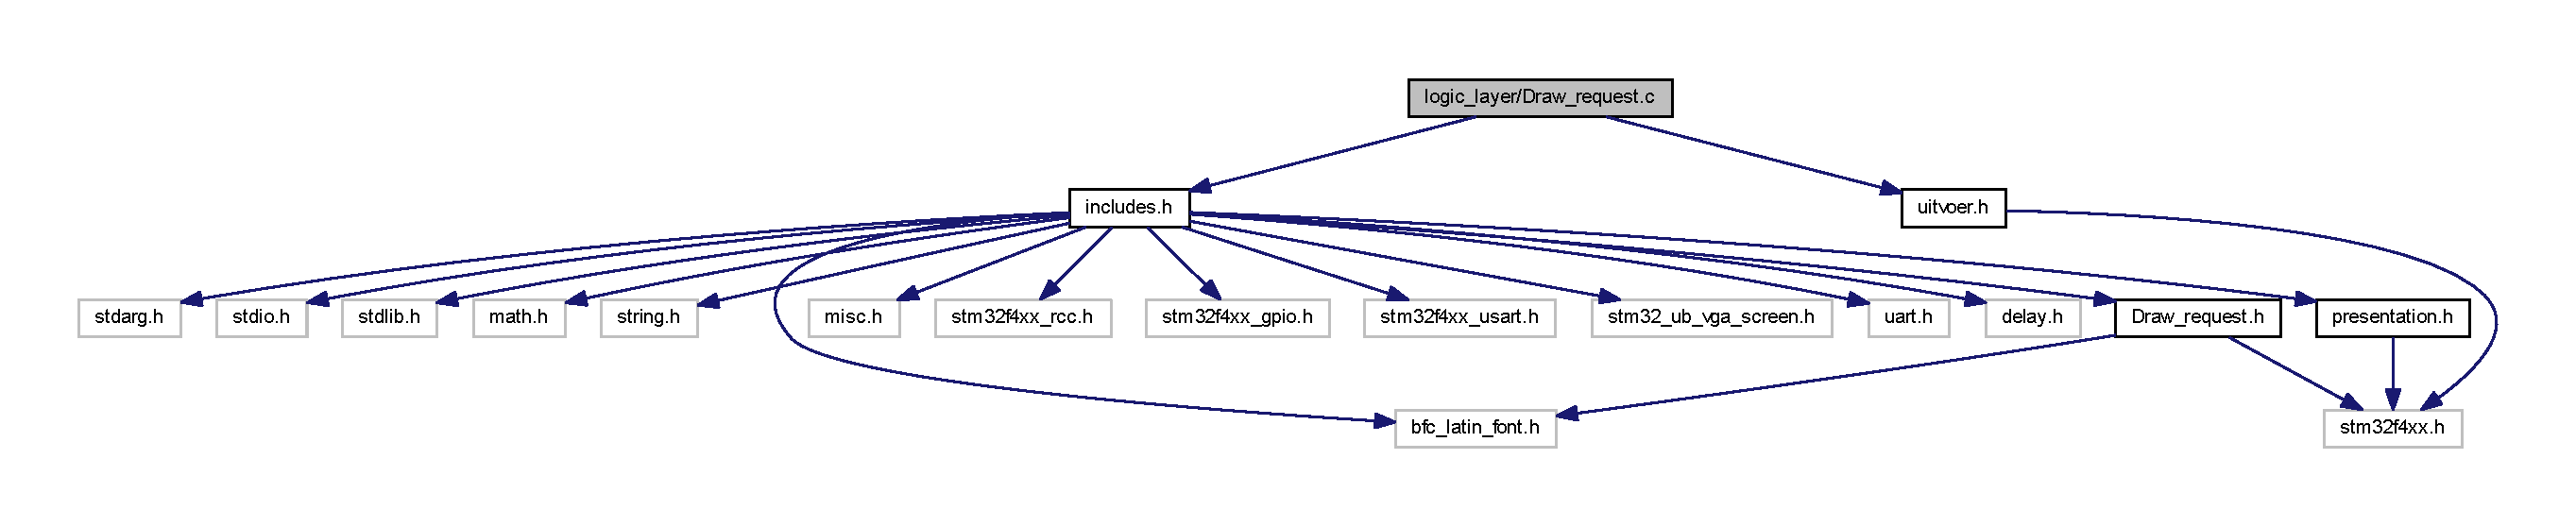
\includegraphics[width=350pt]{_draw__request_8c__incl}
\end{center}
\end{figure}
\subsection*{Functions}
\begin{DoxyCompactItemize}
\item 
void \hyperlink{_draw__request_8c_ab72b41a355531a67fbecd509c90edde9}{T\+I\+M\+E\+R3\+\_\+\+Initialize} ()
\begin{DoxyCompactList}\small\item\em Timer3 Initialization. \end{DoxyCompactList}\item 
void \hyperlink{_draw__request_8c_a36c40ce15fec581ea1d076aea9a41b12}{wait\+\_\+msec} (unsigned int msec)
\item 
signed int \hyperlink{_draw__request_8c_a978257370e90e9832a47bb67a51bcdd0}{Draw\+\_\+\+Line} (uint16\+\_\+t x1, uint16\+\_\+t y1, uint16\+\_\+t x2, uint16\+\_\+t y2, uint8\+\_\+t width, uint8\+\_\+t color)
\begin{DoxyCompactList}\small\item\em Draws a line on a V\+GA screen. \end{DoxyCompactList}\item 
void \hyperlink{_draw__request_8c_a3a0d412ecb4dca2d1c83b65da49bbade}{Draw\+\_\+\+Hor\+Line} (uint16\+\_\+t xp, uint16\+\_\+t yp, uint8\+\_\+t length, uint8\+\_\+t color)
\begin{DoxyCompactList}\small\item\em Draws a horizontal line on a V\+GA screen. \end{DoxyCompactList}\item 
void \hyperlink{_draw__request_8c_a1c72a0e7b90d716ea89145be3b2ac374}{Draw\+\_\+\+Ver\+Line} (uint16\+\_\+t xp, uint16\+\_\+t yp, uint8\+\_\+t length, uint8\+\_\+t color)
\begin{DoxyCompactList}\small\item\em Draws a vertical line on a V\+GA screen. \end{DoxyCompactList}\item 
void \hyperlink{_draw__request_8c_afcc60b34bed9039c997f6d923fb50e4c}{Draw\+\_\+\+Rectangle} (uint16\+\_\+t xp, uint16\+\_\+t yp, uint8\+\_\+t x\+\_\+length, uint8\+\_\+t y\+\_\+length, uint8\+\_\+t line\+\_\+width, uint8\+\_\+t fill, uint8\+\_\+t color)
\begin{DoxyCompactList}\small\item\em Draws a rectangle with any lengths you like on a V\+GA screen. \end{DoxyCompactList}\item 
void \hyperlink{_draw__request_8c_acdbec12042121c8c90b6d2f17d3b1dab}{Draw\+\_\+\+Triangle} (uint16\+\_\+t x1, uint16\+\_\+t y1, uint16\+\_\+t x2, uint16\+\_\+t y2, uint16\+\_\+t x3, uint16\+\_\+t y3, int fill, uint8\+\_\+t line\+\_\+width, uint8\+\_\+t color)
\begin{DoxyCompactList}\small\item\em Draws a triangle with the corners on which ever coordinate you choose. \end{DoxyCompactList}\item 
void \hyperlink{_draw__request_8c_a6f52570e9d95806b556d5d89823dfc38}{Draw\+\_\+\+Ellipse} (uint16\+\_\+t xp, uint16\+\_\+t yp, uint16\+\_\+t r1, uint16\+\_\+t r2, uint16\+\_\+t fill, uint16\+\_\+t thickness, uint8\+\_\+t colour)
\begin{DoxyCompactList}\small\item\em Draws a ellips on a V\+GA screen. \end{DoxyCompactList}\item 
void \hyperlink{_draw__request_8c_aadb59076e96776dbf24e0a6620de0400}{Set\+\_\+\+Single\+\_\+\+Pixel} (uint16\+\_\+t xp, uint16\+\_\+t yp, uint8\+\_\+t colour)
\begin{DoxyCompactList}\small\item\em Colors a pixel on the coordinate of you desire with the color of your desire. \end{DoxyCompactList}\item 
void \hyperlink{_draw__request_8c_a2d4745604fe0ba4c30ad35aeee485cdd}{Clear\+\_\+screen} (uint8\+\_\+t color)
\begin{DoxyCompactList}\small\item\em Turns the whole vga screen into one color. \end{DoxyCompactList}\item 
uint16\+\_\+t \hyperlink{_draw__request_8c_a9dbd751c1ebf034c751ba85222000289}{draw\+\_\+character} (uint16\+\_\+t xp, uint16\+\_\+t yp, int c, uint8\+\_\+t color, \hyperlink{_draw__request_8h_a5f885badaea1ce688c8349bc79e82358}{f\+\_\+name} font\+\_\+name, \hyperlink{_draw__request_8h_afeee049c9120627f4bad4322d131c130}{f\+\_\+type} font\+\_\+type, uint8\+\_\+t font\+\_\+size, uint8\+\_\+t bg)
\begin{DoxyCompactList}\small\item\em Draw a character on the V\+GA screen. \end{DoxyCompactList}\item 
void \hyperlink{_draw__request_8c_ad403fe7bfee17d66ba92bdb7a8d13079}{draw\+\_\+sentence} (uint16\+\_\+t xp, uint16\+\_\+t yp, char $\ast$sent, uint8\+\_\+t color, \hyperlink{_draw__request_8h_a5f885badaea1ce688c8349bc79e82358}{f\+\_\+name} font\+\_\+name, \hyperlink{_draw__request_8h_afeee049c9120627f4bad4322d131c130}{f\+\_\+type} font\+\_\+type, uint8\+\_\+t font\+\_\+size, uint8\+\_\+t bg)
\begin{DoxyCompactList}\small\item\em Draw multiple characyers on the V\+GA screen. \end{DoxyCompactList}\item 
void \hyperlink{_draw__request_8c_a3d61186e3fd07ce89ce81026165499ec}{Bitmap\+\_\+to\+\_\+\+V\+GA} (uint8\+\_\+t image\+\_\+nr, uint8\+\_\+t xp, uint8\+\_\+t yp)
\begin{DoxyCompactList}\small\item\em Draws a the bitmap of a picture/image on a V\+GA screen. \end{DoxyCompactList}\end{DoxyCompactItemize}


\subsection{Function Documentation}
\mbox{\Hypertarget{_draw__request_8c_a3d61186e3fd07ce89ce81026165499ec}\label{_draw__request_8c_a3d61186e3fd07ce89ce81026165499ec}} 
\index{Draw\+\_\+request.\+c@{Draw\+\_\+request.\+c}!Bitmap\+\_\+to\+\_\+\+V\+GA@{Bitmap\+\_\+to\+\_\+\+V\+GA}}
\index{Bitmap\+\_\+to\+\_\+\+V\+GA@{Bitmap\+\_\+to\+\_\+\+V\+GA}!Draw\+\_\+request.\+c@{Draw\+\_\+request.\+c}}
\subsubsection{\texorpdfstring{Bitmap\+\_\+to\+\_\+\+V\+G\+A()}{Bitmap\_to\_VGA()}}
{\footnotesize\ttfamily void Bitmap\+\_\+to\+\_\+\+V\+GA (\begin{DoxyParamCaption}\item[{uint8\+\_\+t}]{image\+\_\+nr,  }\item[{uint8\+\_\+t}]{xp,  }\item[{uint8\+\_\+t}]{yp }\end{DoxyParamCaption})}



Draws a the bitmap of a picture/image on a V\+GA screen. 


\begin{DoxyParams}{Parameters}
{\em image\+\_\+nr} & the number of the image that you want. \\
\hline
{\em xp} & x value of the start coordinate (0 to 320). \\
\hline
{\em yp} & y value of the start coordinate (0 to 240). \\
\hline
\end{DoxyParams}
\begin{DoxyRemark}{Remarks}
{\bfseries Memory} 

{\bfseries Milestone} 
\end{DoxyRemark}
\mbox{\Hypertarget{_draw__request_8c_a2d4745604fe0ba4c30ad35aeee485cdd}\label{_draw__request_8c_a2d4745604fe0ba4c30ad35aeee485cdd}} 
\index{Draw\+\_\+request.\+c@{Draw\+\_\+request.\+c}!Clear\+\_\+screen@{Clear\+\_\+screen}}
\index{Clear\+\_\+screen@{Clear\+\_\+screen}!Draw\+\_\+request.\+c@{Draw\+\_\+request.\+c}}
\subsubsection{\texorpdfstring{Clear\+\_\+screen()}{Clear\_screen()}}
{\footnotesize\ttfamily void Clear\+\_\+screen (\begin{DoxyParamCaption}\item[{uint8\+\_\+t}]{color }\end{DoxyParamCaption})}



Turns the whole vga screen into one color. 


\begin{DoxyParams}{Parameters}
{\em color} & color of the screen(0x00 to 0x\+F\+F). \\
\hline
\end{DoxyParams}
\begin{DoxyRemark}{Remarks}
{\bfseries Memory} 

{\bfseries Milestone} 
\end{DoxyRemark}
\mbox{\Hypertarget{_draw__request_8c_a9dbd751c1ebf034c751ba85222000289}\label{_draw__request_8c_a9dbd751c1ebf034c751ba85222000289}} 
\index{Draw\+\_\+request.\+c@{Draw\+\_\+request.\+c}!draw\+\_\+character@{draw\+\_\+character}}
\index{draw\+\_\+character@{draw\+\_\+character}!Draw\+\_\+request.\+c@{Draw\+\_\+request.\+c}}
\subsubsection{\texorpdfstring{draw\+\_\+character()}{draw\_character()}}
{\footnotesize\ttfamily uint16\+\_\+t draw\+\_\+character (\begin{DoxyParamCaption}\item[{uint16\+\_\+t}]{xp,  }\item[{uint16\+\_\+t}]{yp,  }\item[{int}]{char\+\_\+input,  }\item[{uint8\+\_\+t}]{color,  }\item[{\hyperlink{_draw__request_8h_a5f885badaea1ce688c8349bc79e82358}{f\+\_\+name}}]{font\+\_\+name,  }\item[{\hyperlink{_draw__request_8h_afeee049c9120627f4bad4322d131c130}{f\+\_\+type}}]{font\+\_\+type,  }\item[{uint8\+\_\+t}]{font\+\_\+size,  }\item[{uint8\+\_\+t}]{bg }\end{DoxyParamCaption})}



Draw a character on the V\+GA screen. 


\begin{DoxyParams}{Parameters}
{\em xp} & x value of the pixel coordinate (0 to 320). \\
\hline
{\em yp} & y value of the pixel coordinate (0 to 240). \\
\hline
{\em color} & color of the pixel (0x00 to 0x\+FF). \\
\hline
{\em font\+\_\+name} & \\
\hline
{\em font\+\_\+type} & \\
\hline
{\em font\+\_\+size} & \\
\hline
{\em bg} & background color. \\
\hline
\end{DoxyParams}
\begin{DoxyReturn}{Returns}
char\+\_\+width 
\end{DoxyReturn}
\begin{DoxyRemark}{Remarks}
{\bfseries Memory} 

{\bfseries Milestone} 
\end{DoxyRemark}
\mbox{\Hypertarget{_draw__request_8c_a6f52570e9d95806b556d5d89823dfc38}\label{_draw__request_8c_a6f52570e9d95806b556d5d89823dfc38}} 
\index{Draw\+\_\+request.\+c@{Draw\+\_\+request.\+c}!Draw\+\_\+\+Ellipse@{Draw\+\_\+\+Ellipse}}
\index{Draw\+\_\+\+Ellipse@{Draw\+\_\+\+Ellipse}!Draw\+\_\+request.\+c@{Draw\+\_\+request.\+c}}
\subsubsection{\texorpdfstring{Draw\+\_\+\+Ellipse()}{Draw\_Ellipse()}}
{\footnotesize\ttfamily void Draw\+\_\+\+Ellipse (\begin{DoxyParamCaption}\item[{uint16\+\_\+t}]{xp,  }\item[{uint16\+\_\+t}]{yp,  }\item[{uint16\+\_\+t}]{r1,  }\item[{uint16\+\_\+t}]{r2,  }\item[{uint16\+\_\+t}]{fill,  }\item[{uint16\+\_\+t}]{thickness,  }\item[{uint8\+\_\+t}]{colour }\end{DoxyParamCaption})}



Draws a ellips on a V\+GA screen. 


\begin{DoxyParams}{Parameters}
{\em xp} & x value of the start coordinate (0 to 320). \\
\hline
{\em yp} & y value of the start coordinate (0 to 240). \\
\hline
{\em r2} & \\
\hline
{\em fill} & \\
\hline
{\em thickness} & \\
\hline
{\em colour} & color of the line (0x00 to 0x\+FF). \\
\hline
\end{DoxyParams}
\begin{DoxyRemark}{Remarks}
{\bfseries Memory} 

{\bfseries Milestone} 
\end{DoxyRemark}
\mbox{\Hypertarget{_draw__request_8c_a3a0d412ecb4dca2d1c83b65da49bbade}\label{_draw__request_8c_a3a0d412ecb4dca2d1c83b65da49bbade}} 
\index{Draw\+\_\+request.\+c@{Draw\+\_\+request.\+c}!Draw\+\_\+\+Hor\+Line@{Draw\+\_\+\+Hor\+Line}}
\index{Draw\+\_\+\+Hor\+Line@{Draw\+\_\+\+Hor\+Line}!Draw\+\_\+request.\+c@{Draw\+\_\+request.\+c}}
\subsubsection{\texorpdfstring{Draw\+\_\+\+Hor\+Line()}{Draw\_HorLine()}}
{\footnotesize\ttfamily void Draw\+\_\+\+Hor\+Line (\begin{DoxyParamCaption}\item[{uint16\+\_\+t}]{xp,  }\item[{uint16\+\_\+t}]{yp,  }\item[{uint8\+\_\+t}]{length,  }\item[{uint8\+\_\+t}]{color }\end{DoxyParamCaption})}



Draws a horizontal line on a V\+GA screen. 


\begin{DoxyParams}{Parameters}
{\em xp} & x value of the start coordinate (0 to 320). \\
\hline
{\em yp} & y value of the start coordinate (0 to 240). \\
\hline
{\em length} & amount of pixels that makes the length of the line. \\
\hline
{\em color} & color of the line (0x00 to 0x\+FF). \\
\hline
\end{DoxyParams}
\begin{DoxyRemark}{Remarks}
{\bfseries Memory} 
\end{DoxyRemark}
\mbox{\Hypertarget{_draw__request_8c_a978257370e90e9832a47bb67a51bcdd0}\label{_draw__request_8c_a978257370e90e9832a47bb67a51bcdd0}} 
\index{Draw\+\_\+request.\+c@{Draw\+\_\+request.\+c}!Draw\+\_\+\+Line@{Draw\+\_\+\+Line}}
\index{Draw\+\_\+\+Line@{Draw\+\_\+\+Line}!Draw\+\_\+request.\+c@{Draw\+\_\+request.\+c}}
\subsubsection{\texorpdfstring{Draw\+\_\+\+Line()}{Draw\_Line()}}
{\footnotesize\ttfamily signed int Draw\+\_\+\+Line (\begin{DoxyParamCaption}\item[{uint16\+\_\+t}]{x1,  }\item[{uint16\+\_\+t}]{y1,  }\item[{uint16\+\_\+t}]{x2,  }\item[{uint16\+\_\+t}]{y2,  }\item[{uint8\+\_\+t}]{width,  }\item[{uint8\+\_\+t}]{color }\end{DoxyParamCaption})}



Draws a line on a V\+GA screen. 


\begin{DoxyParams}{Parameters}
{\em x1} & x value of the start coordinate (0 to 320). \\
\hline
{\em y1} & y value of the start coordinate (0 to 240). \\
\hline
{\em x2} & x value of the end coordinate (0 to 320). \\
\hline
{\em y2} & y value of the end coordinate (0 to 240). \\
\hline
{\em width} & indicates the width of the line. \\
\hline
{\em color} & color of the line (0x00 to 0x\+FF). \\
\hline
\end{DoxyParams}
\begin{DoxyRemark}{Remarks}
{\bfseries Memory} 

{\bfseries Milestone} It could be faster without all the mathematical stuff going on. 
\end{DoxyRemark}
Here is the caller graph for this function\+:\nopagebreak
\begin{figure}[H]
\begin{center}
\leavevmode
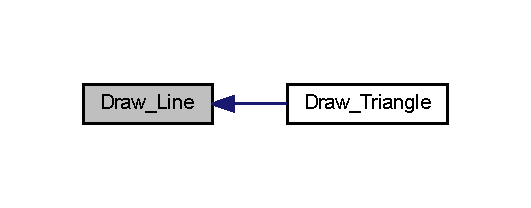
\includegraphics[width=255pt]{_draw__request_8c_a978257370e90e9832a47bb67a51bcdd0_icgraph}
\end{center}
\end{figure}
\mbox{\Hypertarget{_draw__request_8c_afcc60b34bed9039c997f6d923fb50e4c}\label{_draw__request_8c_afcc60b34bed9039c997f6d923fb50e4c}} 
\index{Draw\+\_\+request.\+c@{Draw\+\_\+request.\+c}!Draw\+\_\+\+Rectangle@{Draw\+\_\+\+Rectangle}}
\index{Draw\+\_\+\+Rectangle@{Draw\+\_\+\+Rectangle}!Draw\+\_\+request.\+c@{Draw\+\_\+request.\+c}}
\subsubsection{\texorpdfstring{Draw\+\_\+\+Rectangle()}{Draw\_Rectangle()}}
{\footnotesize\ttfamily void Draw\+\_\+\+Rectangle (\begin{DoxyParamCaption}\item[{uint16\+\_\+t}]{xp,  }\item[{uint16\+\_\+t}]{yp,  }\item[{uint8\+\_\+t}]{x\+\_\+length,  }\item[{uint8\+\_\+t}]{y\+\_\+length,  }\item[{uint8\+\_\+t}]{line\+\_\+width,  }\item[{uint8\+\_\+t}]{fill,  }\item[{uint8\+\_\+t}]{color }\end{DoxyParamCaption})}



Draws a rectangle with any lengths you like on a V\+GA screen. 


\begin{DoxyParams}{Parameters}
{\em xp} & x value of the start coordinate (0 to 320). \\
\hline
{\em yp} & y value of the start coordinate (0 to 240). \\
\hline
{\em x\+\_\+length} & the amount of pixels in the x direction (0 to 320 minus xp). \\
\hline
{\em y\+\_\+length} & the amount of pixels in the y direction (0 to 240 minus yp). \\
\hline
{\em line\+\_\+width} & the width of the drawn line (1 to half of the shortest length). \\
\hline
{\em fill} & filled rectangle (1) or empty rectangle (0). \\
\hline
{\em color} & color of the rectangle (0x00 to 0x\+FF). \\
\hline
\end{DoxyParams}
\begin{DoxyRemark}{Remarks}
{\bfseries Memory} 
\end{DoxyRemark}
\mbox{\Hypertarget{_draw__request_8c_ad403fe7bfee17d66ba92bdb7a8d13079}\label{_draw__request_8c_ad403fe7bfee17d66ba92bdb7a8d13079}} 
\index{Draw\+\_\+request.\+c@{Draw\+\_\+request.\+c}!draw\+\_\+sentence@{draw\+\_\+sentence}}
\index{draw\+\_\+sentence@{draw\+\_\+sentence}!Draw\+\_\+request.\+c@{Draw\+\_\+request.\+c}}
\subsubsection{\texorpdfstring{draw\+\_\+sentence()}{draw\_sentence()}}
{\footnotesize\ttfamily void draw\+\_\+sentence (\begin{DoxyParamCaption}\item[{uint16\+\_\+t}]{xp,  }\item[{uint16\+\_\+t}]{yp,  }\item[{char $\ast$}]{sent,  }\item[{uint8\+\_\+t}]{color,  }\item[{\hyperlink{_draw__request_8h_a5f885badaea1ce688c8349bc79e82358}{f\+\_\+name}}]{font\+\_\+name,  }\item[{\hyperlink{_draw__request_8h_afeee049c9120627f4bad4322d131c130}{f\+\_\+type}}]{font\+\_\+type,  }\item[{uint8\+\_\+t}]{font\+\_\+size,  }\item[{uint8\+\_\+t}]{bg }\end{DoxyParamCaption})}



Draw multiple characyers on the V\+GA screen. 


\begin{DoxyParams}{Parameters}
{\em xp} & x value of the pixel coordinate (0 to 320). \\
\hline
{\em yp} & y value of the pixel coordinate (0 to 240). \\
\hline
{\em color} & color of the pixel (0x00 to 0x\+FF). \\
\hline
{\em font\+\_\+name} & \\
\hline
{\em font\+\_\+type} & \\
\hline
{\em font\+\_\+size} & \\
\hline
{\em bg} & background color. \\
\hline
\end{DoxyParams}
\begin{DoxyRemark}{Remarks}
{\bfseries Memory} 

{\bfseries Milestone} 
\end{DoxyRemark}
\mbox{\Hypertarget{_draw__request_8c_acdbec12042121c8c90b6d2f17d3b1dab}\label{_draw__request_8c_acdbec12042121c8c90b6d2f17d3b1dab}} 
\index{Draw\+\_\+request.\+c@{Draw\+\_\+request.\+c}!Draw\+\_\+\+Triangle@{Draw\+\_\+\+Triangle}}
\index{Draw\+\_\+\+Triangle@{Draw\+\_\+\+Triangle}!Draw\+\_\+request.\+c@{Draw\+\_\+request.\+c}}
\subsubsection{\texorpdfstring{Draw\+\_\+\+Triangle()}{Draw\_Triangle()}}
{\footnotesize\ttfamily void void Draw\+\_\+\+Triangle (\begin{DoxyParamCaption}\item[{uint16\+\_\+t}]{x1,  }\item[{uint16\+\_\+t}]{y1,  }\item[{uint16\+\_\+t}]{x2,  }\item[{uint16\+\_\+t}]{y2,  }\item[{uint16\+\_\+t}]{x3,  }\item[{uint16\+\_\+t}]{y3,  }\item[{int}]{fill,  }\item[{uint8\+\_\+t}]{line\+\_\+width,  }\item[{uint8\+\_\+t}]{color }\end{DoxyParamCaption})}



Draws a triangle with the corners on which ever coordinate you choose. 


\begin{DoxyParams}{Parameters}
{\em x1} & x value of the first coordinate (0 to 320). \\
\hline
{\em y1} & y value of the first coordinate (0 to 240). \\
\hline
{\em x2} & x value of the second coordinate (0 to 320). \\
\hline
{\em y2} & y value of the second coordinate (0 to 240). \\
\hline
{\em x3} & x value of the third coordinate (0 to 320). \\
\hline
{\em y3} & y value of the third coordinate (0 to 240). \\
\hline
{\em fill} & filled triangle (1) or empty triangle (0). \\
\hline
{\em color} & color of the triangle (0x00 to 0x\+FF). \\
\hline
\end{DoxyParams}
\begin{DoxyRemark}{Remarks}
{\bfseries Memory} 

{\bfseries Milestone} It could be faster without all the mathematical stuff going on. 
\end{DoxyRemark}
Here is the call graph for this function\+:\nopagebreak
\begin{figure}[H]
\begin{center}
\leavevmode
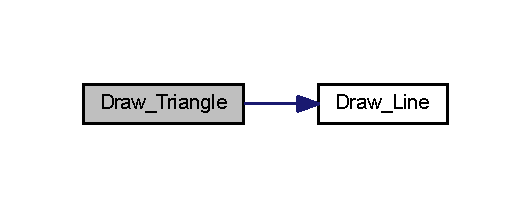
\includegraphics[width=255pt]{_draw__request_8c_acdbec12042121c8c90b6d2f17d3b1dab_cgraph}
\end{center}
\end{figure}
\mbox{\Hypertarget{_draw__request_8c_a1c72a0e7b90d716ea89145be3b2ac374}\label{_draw__request_8c_a1c72a0e7b90d716ea89145be3b2ac374}} 
\index{Draw\+\_\+request.\+c@{Draw\+\_\+request.\+c}!Draw\+\_\+\+Ver\+Line@{Draw\+\_\+\+Ver\+Line}}
\index{Draw\+\_\+\+Ver\+Line@{Draw\+\_\+\+Ver\+Line}!Draw\+\_\+request.\+c@{Draw\+\_\+request.\+c}}
\subsubsection{\texorpdfstring{Draw\+\_\+\+Ver\+Line()}{Draw\_VerLine()}}
{\footnotesize\ttfamily void Draw\+\_\+\+Ver\+Line (\begin{DoxyParamCaption}\item[{uint16\+\_\+t}]{xp,  }\item[{uint16\+\_\+t}]{yp,  }\item[{uint8\+\_\+t}]{length,  }\item[{uint8\+\_\+t}]{color }\end{DoxyParamCaption})}



Draws a vertical line on a V\+GA screen. 


\begin{DoxyParams}{Parameters}
{\em xp} & x value of the start coordinate (0 to 320). \\
\hline
{\em yp} & y value of the start coordinate (0 to 240). \\
\hline
{\em length} & amount of pixels that makes the length of the line. \\
\hline
{\em color} & color of the line (0x00 to 0x\+FF). \\
\hline
\end{DoxyParams}
\begin{DoxyRemark}{Remarks}
{\bfseries Memory} 
\end{DoxyRemark}
\mbox{\Hypertarget{_draw__request_8c_aadb59076e96776dbf24e0a6620de0400}\label{_draw__request_8c_aadb59076e96776dbf24e0a6620de0400}} 
\index{Draw\+\_\+request.\+c@{Draw\+\_\+request.\+c}!Set\+\_\+\+Single\+\_\+\+Pixel@{Set\+\_\+\+Single\+\_\+\+Pixel}}
\index{Set\+\_\+\+Single\+\_\+\+Pixel@{Set\+\_\+\+Single\+\_\+\+Pixel}!Draw\+\_\+request.\+c@{Draw\+\_\+request.\+c}}
\subsubsection{\texorpdfstring{Set\+\_\+\+Single\+\_\+\+Pixel()}{Set\_Single\_Pixel()}}
{\footnotesize\ttfamily void Set\+\_\+\+Single\+\_\+\+Pixel (\begin{DoxyParamCaption}\item[{uint16\+\_\+t}]{xp,  }\item[{uint16\+\_\+t}]{yp,  }\item[{uint8\+\_\+t}]{colour }\end{DoxyParamCaption})}



Colors a pixel on the coordinate of you desire with the color of your desire. 


\begin{DoxyParams}{Parameters}
{\em xp} & x value of the pixel coordinate (0 to 320). \\
\hline
{\em yp} & y value of the pixel coordinate (0 to 240). \\
\hline
{\em color} & color of the pixel (0x00 to 0x\+FF). \\
\hline
\end{DoxyParams}
\begin{DoxyRemark}{Remarks}
{\bfseries Memory} 

{\bfseries Milestone} 
\end{DoxyRemark}
\mbox{\Hypertarget{_draw__request_8c_ab72b41a355531a67fbecd509c90edde9}\label{_draw__request_8c_ab72b41a355531a67fbecd509c90edde9}} 
\index{Draw\+\_\+request.\+c@{Draw\+\_\+request.\+c}!T\+I\+M\+E\+R3\+\_\+\+Initialize@{T\+I\+M\+E\+R3\+\_\+\+Initialize}}
\index{T\+I\+M\+E\+R3\+\_\+\+Initialize@{T\+I\+M\+E\+R3\+\_\+\+Initialize}!Draw\+\_\+request.\+c@{Draw\+\_\+request.\+c}}
\subsubsection{\texorpdfstring{T\+I\+M\+E\+R3\+\_\+\+Initialize()}{TIMER3\_Initialize()}}
{\footnotesize\ttfamily void T\+I\+M\+E\+R3\+\_\+\+Initialize (\begin{DoxyParamCaption}{ }\end{DoxyParamCaption})}



Timer3 Initialization. 

Here is the caller graph for this function\+:\nopagebreak
\begin{figure}[H]
\begin{center}
\leavevmode
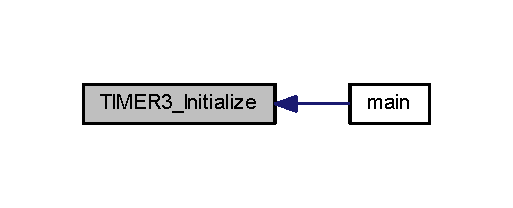
\includegraphics[width=246pt]{_draw__request_8c_ab72b41a355531a67fbecd509c90edde9_icgraph}
\end{center}
\end{figure}
\mbox{\Hypertarget{_draw__request_8c_a36c40ce15fec581ea1d076aea9a41b12}\label{_draw__request_8c_a36c40ce15fec581ea1d076aea9a41b12}} 
\index{Draw\+\_\+request.\+c@{Draw\+\_\+request.\+c}!wait\+\_\+msec@{wait\+\_\+msec}}
\index{wait\+\_\+msec@{wait\+\_\+msec}!Draw\+\_\+request.\+c@{Draw\+\_\+request.\+c}}
\subsubsection{\texorpdfstring{wait\+\_\+msec()}{wait\_msec()}}
{\footnotesize\ttfamily void wait\+\_\+msec (\begin{DoxyParamCaption}\item[{unsigned int}]{msec }\end{DoxyParamCaption})}


\begin{DoxyParams}{Parameters}
{\em msec} & \\
\hline
\end{DoxyParams}
\begin{DoxyRemark}{Remarks}
Memory\+: 

Wat kan er beter? 
\end{DoxyRemark}

\hypertarget{_draw__request_8h}{}\section{logic\+\_\+layer/\+Draw\+\_\+request.h File Reference}
\label{_draw__request_8h}\index{logic\+\_\+layer/\+Draw\+\_\+request.\+h@{logic\+\_\+layer/\+Draw\+\_\+request.\+h}}
{\ttfamily \#include \char`\"{}stm32f4xx.\+h\char`\"{}}\newline
{\ttfamily \#include \char`\"{}bfc\+\_\+latin\+\_\+font.\+h\char`\"{}}\newline
Include dependency graph for Draw\+\_\+request.\+h\+:\nopagebreak
\begin{figure}[H]
\begin{center}
\leavevmode
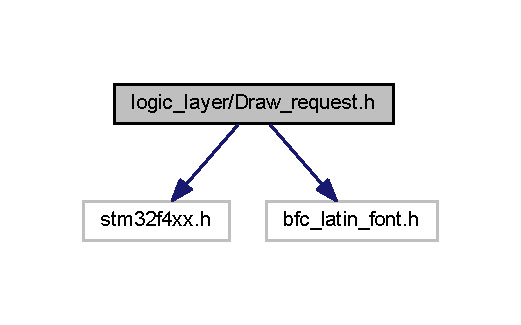
\includegraphics[width=250pt]{_draw__request_8h__incl}
\end{center}
\end{figure}
This graph shows which files directly or indirectly include this file\+:\nopagebreak
\begin{figure}[H]
\begin{center}
\leavevmode
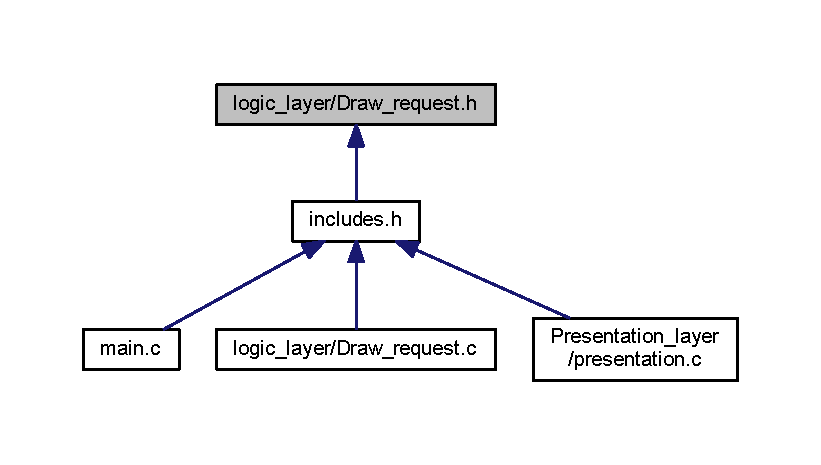
\includegraphics[width=350pt]{_draw__request_8h__dep__incl}
\end{center}
\end{figure}
\subsection*{Macros}
\begin{DoxyCompactItemize}
\item 
\#define \hyperlink{_draw__request_8h_a598a3330b3c21701223ee0ca14316eca}{PI}~3.\+14159265359
\item 
\#define \hyperlink{_draw__request_8h_acf926951944b6cf370b7229ebd50dd8b}{T\+I\+M\+E\+R\+\_\+\+F\+R\+EQ}~1000
\item 
\#define \hyperlink{_draw__request_8h_ab3a7892b9f9fbb5c3fc2cbdbceb10017}{S\+Y\+S\+\_\+\+C\+LK}~168000000
\end{DoxyCompactItemize}
\subsection*{Enumerations}
\begin{DoxyCompactItemize}
\item 
enum \hyperlink{_draw__request_8h_a5f885badaea1ce688c8349bc79e82358}{f\+\_\+name} \{ \hyperlink{_draw__request_8h_a5f885badaea1ce688c8349bc79e82358ab143123bd6490db2cf41321660fadebd}{Times\+\_\+\+New\+\_\+\+Roman}, 
\hyperlink{_draw__request_8h_a5f885badaea1ce688c8349bc79e82358a9b5cabe795112055e76ea03101f43ec8}{Georgia}
 \}
\item 
enum \hyperlink{_draw__request_8h_afeee049c9120627f4bad4322d131c130}{f\+\_\+type} \{ \hyperlink{_draw__request_8h_afeee049c9120627f4bad4322d131c130ac69b11a9431062a98e634b1a67db479c}{bold}, 
\hyperlink{_draw__request_8h_afeee049c9120627f4bad4322d131c130a040a9ec6d2966f099fd3214b8ac4fef3}{regular}
 \}
\end{DoxyCompactItemize}
\subsection*{Functions}
\begin{DoxyCompactItemize}
\item 
void \hyperlink{_draw__request_8h_ab72b41a355531a67fbecd509c90edde9}{T\+I\+M\+E\+R3\+\_\+\+Initialize} ()
\begin{DoxyCompactList}\small\item\em Timer3 Initialization. \end{DoxyCompactList}\item 
void \hyperlink{_draw__request_8h_a36c40ce15fec581ea1d076aea9a41b12}{wait\+\_\+msec} (unsigned int msec)
\item 
void \hyperlink{_draw__request_8h_a6f52570e9d95806b556d5d89823dfc38}{Draw\+\_\+\+Ellipse} (uint16\+\_\+t xp, uint16\+\_\+t yp, uint16\+\_\+t r1, uint16\+\_\+t r2, uint16\+\_\+t fill, uint16\+\_\+t thickness, uint8\+\_\+t colour)
\begin{DoxyCompactList}\small\item\em Draws a ellips on a V\+GA screen. \end{DoxyCompactList}\item 
void \hyperlink{_draw__request_8h_a2d4745604fe0ba4c30ad35aeee485cdd}{Clear\+\_\+screen} (uint8\+\_\+t color)
\begin{DoxyCompactList}\small\item\em Turns the whole vga screen into one color. \end{DoxyCompactList}\item 
void \hyperlink{_draw__request_8h_a3d61186e3fd07ce89ce81026165499ec}{Bitmap\+\_\+to\+\_\+\+V\+GA} (uint8\+\_\+t image\+\_\+nr, uint8\+\_\+t xp, uint8\+\_\+t yp)
\begin{DoxyCompactList}\small\item\em Draws a the bitmap of a picture/image on a V\+GA screen. \end{DoxyCompactList}\item 
signed int \hyperlink{_draw__request_8h_a978257370e90e9832a47bb67a51bcdd0}{Draw\+\_\+\+Line} (uint16\+\_\+t x1, uint16\+\_\+t y1, uint16\+\_\+t x2, uint16\+\_\+t y2, uint8\+\_\+t width, uint8\+\_\+t color)
\begin{DoxyCompactList}\small\item\em Draws a line on a V\+GA screen. \end{DoxyCompactList}\item 
void \hyperlink{_draw__request_8h_a3a0d412ecb4dca2d1c83b65da49bbade}{Draw\+\_\+\+Hor\+Line} (uint16\+\_\+t xp, uint16\+\_\+t yp, uint8\+\_\+t length, uint8\+\_\+t color)
\begin{DoxyCompactList}\small\item\em Draws a horizontal line on a V\+GA screen. \end{DoxyCompactList}\item 
void \hyperlink{_draw__request_8h_a1c72a0e7b90d716ea89145be3b2ac374}{Draw\+\_\+\+Ver\+Line} (uint16\+\_\+t xp, uint16\+\_\+t yp, uint8\+\_\+t length, uint8\+\_\+t color)
\begin{DoxyCompactList}\small\item\em Draws a vertical line on a V\+GA screen. \end{DoxyCompactList}\item 
void \hyperlink{_draw__request_8h_afcc60b34bed9039c997f6d923fb50e4c}{Draw\+\_\+\+Rectangle} (uint16\+\_\+t xp, uint16\+\_\+t yp, uint8\+\_\+t x\+\_\+length, uint8\+\_\+t y\+\_\+length, uint8\+\_\+t line\+\_\+width, uint8\+\_\+t fill, uint8\+\_\+t color)
\begin{DoxyCompactList}\small\item\em Draws a rectangle with any lengths you like on a V\+GA screen. \end{DoxyCompactList}\item 
void \hyperlink{_draw__request_8h_a6d2f3b22c1ae88122730df5de2981cd7}{Draw\+\_\+\+Triangle} (uint16\+\_\+t x1, uint16\+\_\+t y1, uint16\+\_\+t x2, uint16\+\_\+t y2, uint16\+\_\+t x3, uint16\+\_\+t y3, int fill, uint8\+\_\+t line\+\_\+width, uint8\+\_\+t color)
\begin{DoxyCompactList}\small\item\em Draws a triangle with the corners on which ever coordinate you choose. \end{DoxyCompactList}\item 
void \hyperlink{_draw__request_8h_aadb59076e96776dbf24e0a6620de0400}{Set\+\_\+\+Single\+\_\+\+Pixel} (uint16\+\_\+t xp, uint16\+\_\+t yp, uint8\+\_\+t colour)
\begin{DoxyCompactList}\small\item\em Colors a pixel on the coordinate of you desire with the color of your desire. \end{DoxyCompactList}\item 
uint16\+\_\+t \hyperlink{_draw__request_8h_a360c2168c1ae121c870bcad27626b978}{draw\+\_\+character} (uint16\+\_\+t xp, uint16\+\_\+t yp, int char\+\_\+input, uint8\+\_\+t color, \hyperlink{_draw__request_8h_a5f885badaea1ce688c8349bc79e82358}{f\+\_\+name} font\+\_\+name, \hyperlink{_draw__request_8h_afeee049c9120627f4bad4322d131c130}{f\+\_\+type} font\+\_\+type, uint8\+\_\+t font\+\_\+size, uint8\+\_\+t bg)
\begin{DoxyCompactList}\small\item\em Draw a character on the V\+GA screen. \end{DoxyCompactList}\item 
void \hyperlink{_draw__request_8h_ad403fe7bfee17d66ba92bdb7a8d13079}{draw\+\_\+sentence} (uint16\+\_\+t xp, uint16\+\_\+t yp, char $\ast$sent, uint8\+\_\+t color, \hyperlink{_draw__request_8h_a5f885badaea1ce688c8349bc79e82358}{f\+\_\+name} font\+\_\+name, \hyperlink{_draw__request_8h_afeee049c9120627f4bad4322d131c130}{f\+\_\+type} font\+\_\+type, uint8\+\_\+t font\+\_\+size, uint8\+\_\+t bg)
\begin{DoxyCompactList}\small\item\em Draw multiple characyers on the V\+GA screen. \end{DoxyCompactList}\end{DoxyCompactItemize}


\subsection{Macro Definition Documentation}
\mbox{\Hypertarget{_draw__request_8h_a598a3330b3c21701223ee0ca14316eca}\label{_draw__request_8h_a598a3330b3c21701223ee0ca14316eca}} 
\index{Draw\+\_\+request.\+h@{Draw\+\_\+request.\+h}!PI@{PI}}
\index{PI@{PI}!Draw\+\_\+request.\+h@{Draw\+\_\+request.\+h}}
\subsubsection{\texorpdfstring{PI}{PI}}
{\footnotesize\ttfamily \#define PI~3.\+14159265359}

\mbox{\Hypertarget{_draw__request_8h_ab3a7892b9f9fbb5c3fc2cbdbceb10017}\label{_draw__request_8h_ab3a7892b9f9fbb5c3fc2cbdbceb10017}} 
\index{Draw\+\_\+request.\+h@{Draw\+\_\+request.\+h}!S\+Y\+S\+\_\+\+C\+LK@{S\+Y\+S\+\_\+\+C\+LK}}
\index{S\+Y\+S\+\_\+\+C\+LK@{S\+Y\+S\+\_\+\+C\+LK}!Draw\+\_\+request.\+h@{Draw\+\_\+request.\+h}}
\subsubsection{\texorpdfstring{S\+Y\+S\+\_\+\+C\+LK}{SYS\_CLK}}
{\footnotesize\ttfamily \#define S\+Y\+S\+\_\+\+C\+LK~168000000}

\mbox{\Hypertarget{_draw__request_8h_acf926951944b6cf370b7229ebd50dd8b}\label{_draw__request_8h_acf926951944b6cf370b7229ebd50dd8b}} 
\index{Draw\+\_\+request.\+h@{Draw\+\_\+request.\+h}!T\+I\+M\+E\+R\+\_\+\+F\+R\+EQ@{T\+I\+M\+E\+R\+\_\+\+F\+R\+EQ}}
\index{T\+I\+M\+E\+R\+\_\+\+F\+R\+EQ@{T\+I\+M\+E\+R\+\_\+\+F\+R\+EQ}!Draw\+\_\+request.\+h@{Draw\+\_\+request.\+h}}
\subsubsection{\texorpdfstring{T\+I\+M\+E\+R\+\_\+\+F\+R\+EQ}{TIMER\_FREQ}}
{\footnotesize\ttfamily \#define T\+I\+M\+E\+R\+\_\+\+F\+R\+EQ~1000}



\subsection{Enumeration Type Documentation}
\mbox{\Hypertarget{_draw__request_8h_a5f885badaea1ce688c8349bc79e82358}\label{_draw__request_8h_a5f885badaea1ce688c8349bc79e82358}} 
\index{Draw\+\_\+request.\+h@{Draw\+\_\+request.\+h}!f\+\_\+name@{f\+\_\+name}}
\index{f\+\_\+name@{f\+\_\+name}!Draw\+\_\+request.\+h@{Draw\+\_\+request.\+h}}
\subsubsection{\texorpdfstring{f\+\_\+name}{f\_name}}
{\footnotesize\ttfamily enum \hyperlink{_draw__request_8h_a5f885badaea1ce688c8349bc79e82358}{f\+\_\+name}}

\begin{DoxyEnumFields}{Enumerator}
\raisebox{\heightof{T}}[0pt][0pt]{\index{Times\+\_\+\+New\+\_\+\+Roman@{Times\+\_\+\+New\+\_\+\+Roman}!Draw\+\_\+request.\+h@{Draw\+\_\+request.\+h}}\index{Draw\+\_\+request.\+h@{Draw\+\_\+request.\+h}!Times\+\_\+\+New\+\_\+\+Roman@{Times\+\_\+\+New\+\_\+\+Roman}}}\mbox{\Hypertarget{_draw__request_8h_a5f885badaea1ce688c8349bc79e82358ab143123bd6490db2cf41321660fadebd}\label{_draw__request_8h_a5f885badaea1ce688c8349bc79e82358ab143123bd6490db2cf41321660fadebd}} 
Times\+\_\+\+New\+\_\+\+Roman&\\
\hline

\raisebox{\heightof{T}}[0pt][0pt]{\index{Georgia@{Georgia}!Draw\+\_\+request.\+h@{Draw\+\_\+request.\+h}}\index{Draw\+\_\+request.\+h@{Draw\+\_\+request.\+h}!Georgia@{Georgia}}}\mbox{\Hypertarget{_draw__request_8h_a5f885badaea1ce688c8349bc79e82358a9b5cabe795112055e76ea03101f43ec8}\label{_draw__request_8h_a5f885badaea1ce688c8349bc79e82358a9b5cabe795112055e76ea03101f43ec8}} 
Georgia&\\
\hline

\end{DoxyEnumFields}
\mbox{\Hypertarget{_draw__request_8h_afeee049c9120627f4bad4322d131c130}\label{_draw__request_8h_afeee049c9120627f4bad4322d131c130}} 
\index{Draw\+\_\+request.\+h@{Draw\+\_\+request.\+h}!f\+\_\+type@{f\+\_\+type}}
\index{f\+\_\+type@{f\+\_\+type}!Draw\+\_\+request.\+h@{Draw\+\_\+request.\+h}}
\subsubsection{\texorpdfstring{f\+\_\+type}{f\_type}}
{\footnotesize\ttfamily enum \hyperlink{_draw__request_8h_afeee049c9120627f4bad4322d131c130}{f\+\_\+type}}

\begin{DoxyEnumFields}{Enumerator}
\raisebox{\heightof{T}}[0pt][0pt]{\index{bold@{bold}!Draw\+\_\+request.\+h@{Draw\+\_\+request.\+h}}\index{Draw\+\_\+request.\+h@{Draw\+\_\+request.\+h}!bold@{bold}}}\mbox{\Hypertarget{_draw__request_8h_afeee049c9120627f4bad4322d131c130ac69b11a9431062a98e634b1a67db479c}\label{_draw__request_8h_afeee049c9120627f4bad4322d131c130ac69b11a9431062a98e634b1a67db479c}} 
bold&\\
\hline

\raisebox{\heightof{T}}[0pt][0pt]{\index{regular@{regular}!Draw\+\_\+request.\+h@{Draw\+\_\+request.\+h}}\index{Draw\+\_\+request.\+h@{Draw\+\_\+request.\+h}!regular@{regular}}}\mbox{\Hypertarget{_draw__request_8h_afeee049c9120627f4bad4322d131c130a040a9ec6d2966f099fd3214b8ac4fef3}\label{_draw__request_8h_afeee049c9120627f4bad4322d131c130a040a9ec6d2966f099fd3214b8ac4fef3}} 
regular&\\
\hline

\end{DoxyEnumFields}


\subsection{Function Documentation}
\mbox{\Hypertarget{_draw__request_8h_a3d61186e3fd07ce89ce81026165499ec}\label{_draw__request_8h_a3d61186e3fd07ce89ce81026165499ec}} 
\index{Draw\+\_\+request.\+h@{Draw\+\_\+request.\+h}!Bitmap\+\_\+to\+\_\+\+V\+GA@{Bitmap\+\_\+to\+\_\+\+V\+GA}}
\index{Bitmap\+\_\+to\+\_\+\+V\+GA@{Bitmap\+\_\+to\+\_\+\+V\+GA}!Draw\+\_\+request.\+h@{Draw\+\_\+request.\+h}}
\subsubsection{\texorpdfstring{Bitmap\+\_\+to\+\_\+\+V\+G\+A()}{Bitmap\_to\_VGA()}}
{\footnotesize\ttfamily void Bitmap\+\_\+to\+\_\+\+V\+GA (\begin{DoxyParamCaption}\item[{uint8\+\_\+t}]{image\+\_\+nr,  }\item[{uint8\+\_\+t}]{xp,  }\item[{uint8\+\_\+t}]{yp }\end{DoxyParamCaption})}



Draws a the bitmap of a picture/image on a V\+GA screen. 


\begin{DoxyParams}{Parameters}
{\em image\+\_\+nr} & the number of the image that you want. \\
\hline
{\em xp} & x value of the start coordinate (0 to 320). \\
\hline
{\em yp} & y value of the start coordinate (0 to 240). \\
\hline
\end{DoxyParams}
\begin{DoxyRemark}{Remarks}
{\bfseries Memory} 

{\bfseries Milestone} 
\end{DoxyRemark}
\mbox{\Hypertarget{_draw__request_8h_a2d4745604fe0ba4c30ad35aeee485cdd}\label{_draw__request_8h_a2d4745604fe0ba4c30ad35aeee485cdd}} 
\index{Draw\+\_\+request.\+h@{Draw\+\_\+request.\+h}!Clear\+\_\+screen@{Clear\+\_\+screen}}
\index{Clear\+\_\+screen@{Clear\+\_\+screen}!Draw\+\_\+request.\+h@{Draw\+\_\+request.\+h}}
\subsubsection{\texorpdfstring{Clear\+\_\+screen()}{Clear\_screen()}}
{\footnotesize\ttfamily void Clear\+\_\+screen (\begin{DoxyParamCaption}\item[{uint8\+\_\+t}]{color }\end{DoxyParamCaption})}



Turns the whole vga screen into one color. 


\begin{DoxyParams}{Parameters}
{\em color} & color of the screen(0x00 to 0x\+F\+F). \\
\hline
\end{DoxyParams}
\begin{DoxyRemark}{Remarks}
{\bfseries Memory} 

{\bfseries Milestone} 
\end{DoxyRemark}
\mbox{\Hypertarget{_draw__request_8h_a360c2168c1ae121c870bcad27626b978}\label{_draw__request_8h_a360c2168c1ae121c870bcad27626b978}} 
\index{Draw\+\_\+request.\+h@{Draw\+\_\+request.\+h}!draw\+\_\+character@{draw\+\_\+character}}
\index{draw\+\_\+character@{draw\+\_\+character}!Draw\+\_\+request.\+h@{Draw\+\_\+request.\+h}}
\subsubsection{\texorpdfstring{draw\+\_\+character()}{draw\_character()}}
{\footnotesize\ttfamily uint16\+\_\+t draw\+\_\+character (\begin{DoxyParamCaption}\item[{uint16\+\_\+t}]{xp,  }\item[{uint16\+\_\+t}]{yp,  }\item[{int}]{c,  }\item[{uint8\+\_\+t}]{color,  }\item[{\hyperlink{_draw__request_8h_a5f885badaea1ce688c8349bc79e82358}{f\+\_\+name}}]{font\+\_\+name,  }\item[{\hyperlink{_draw__request_8h_afeee049c9120627f4bad4322d131c130}{f\+\_\+type}}]{font\+\_\+type,  }\item[{uint8\+\_\+t}]{font\+\_\+size,  }\item[{uint8\+\_\+t}]{bg }\end{DoxyParamCaption})}



Draw a character on the V\+GA screen. 


\begin{DoxyParams}{Parameters}
{\em xp} & x value of the pixel coordinate (0 to 320). \\
\hline
{\em yp} & y value of the pixel coordinate (0 to 240). \\
\hline
{\em color} & color of the pixel (0x00 to 0x\+FF). \\
\hline
{\em font\+\_\+name} & \\
\hline
{\em font\+\_\+type} & \\
\hline
{\em font\+\_\+size} & \\
\hline
{\em bg} & background color. \\
\hline
\end{DoxyParams}
\begin{DoxyReturn}{Returns}
char\+\_\+width 
\end{DoxyReturn}
\begin{DoxyRemark}{Remarks}
{\bfseries Memory} 

{\bfseries Milestone} 
\end{DoxyRemark}
\mbox{\Hypertarget{_draw__request_8h_a6f52570e9d95806b556d5d89823dfc38}\label{_draw__request_8h_a6f52570e9d95806b556d5d89823dfc38}} 
\index{Draw\+\_\+request.\+h@{Draw\+\_\+request.\+h}!Draw\+\_\+\+Ellipse@{Draw\+\_\+\+Ellipse}}
\index{Draw\+\_\+\+Ellipse@{Draw\+\_\+\+Ellipse}!Draw\+\_\+request.\+h@{Draw\+\_\+request.\+h}}
\subsubsection{\texorpdfstring{Draw\+\_\+\+Ellipse()}{Draw\_Ellipse()}}
{\footnotesize\ttfamily void Draw\+\_\+\+Ellipse (\begin{DoxyParamCaption}\item[{uint16\+\_\+t}]{xp,  }\item[{uint16\+\_\+t}]{yp,  }\item[{uint16\+\_\+t}]{r1,  }\item[{uint16\+\_\+t}]{r2,  }\item[{uint16\+\_\+t}]{fill,  }\item[{uint16\+\_\+t}]{thickness,  }\item[{uint8\+\_\+t}]{colour }\end{DoxyParamCaption})}



Draws a ellips on a V\+GA screen. 


\begin{DoxyParams}{Parameters}
{\em xp} & x value of the start coordinate (0 to 320). \\
\hline
{\em yp} & y value of the start coordinate (0 to 240). \\
\hline
{\em r2} & \\
\hline
{\em fill} & \\
\hline
{\em thickness} & \\
\hline
{\em colour} & color of the line (0x00 to 0x\+FF). \\
\hline
\end{DoxyParams}
\begin{DoxyRemark}{Remarks}
{\bfseries Memory} 

{\bfseries Milestone} 
\end{DoxyRemark}
\mbox{\Hypertarget{_draw__request_8h_a3a0d412ecb4dca2d1c83b65da49bbade}\label{_draw__request_8h_a3a0d412ecb4dca2d1c83b65da49bbade}} 
\index{Draw\+\_\+request.\+h@{Draw\+\_\+request.\+h}!Draw\+\_\+\+Hor\+Line@{Draw\+\_\+\+Hor\+Line}}
\index{Draw\+\_\+\+Hor\+Line@{Draw\+\_\+\+Hor\+Line}!Draw\+\_\+request.\+h@{Draw\+\_\+request.\+h}}
\subsubsection{\texorpdfstring{Draw\+\_\+\+Hor\+Line()}{Draw\_HorLine()}}
{\footnotesize\ttfamily void Draw\+\_\+\+Hor\+Line (\begin{DoxyParamCaption}\item[{uint16\+\_\+t}]{xp,  }\item[{uint16\+\_\+t}]{yp,  }\item[{uint8\+\_\+t}]{length,  }\item[{uint8\+\_\+t}]{color }\end{DoxyParamCaption})}



Draws a horizontal line on a V\+GA screen. 


\begin{DoxyParams}{Parameters}
{\em xp} & x value of the start coordinate (0 to 320). \\
\hline
{\em yp} & y value of the start coordinate (0 to 240). \\
\hline
{\em length} & amount of pixels that makes the length of the line. \\
\hline
{\em color} & color of the line (0x00 to 0x\+FF). \\
\hline
\end{DoxyParams}
\begin{DoxyRemark}{Remarks}
{\bfseries Memory} 
\end{DoxyRemark}
\mbox{\Hypertarget{_draw__request_8h_a978257370e90e9832a47bb67a51bcdd0}\label{_draw__request_8h_a978257370e90e9832a47bb67a51bcdd0}} 
\index{Draw\+\_\+request.\+h@{Draw\+\_\+request.\+h}!Draw\+\_\+\+Line@{Draw\+\_\+\+Line}}
\index{Draw\+\_\+\+Line@{Draw\+\_\+\+Line}!Draw\+\_\+request.\+h@{Draw\+\_\+request.\+h}}
\subsubsection{\texorpdfstring{Draw\+\_\+\+Line()}{Draw\_Line()}}
{\footnotesize\ttfamily signed int Draw\+\_\+\+Line (\begin{DoxyParamCaption}\item[{uint16\+\_\+t}]{x1,  }\item[{uint16\+\_\+t}]{y1,  }\item[{uint16\+\_\+t}]{x2,  }\item[{uint16\+\_\+t}]{y2,  }\item[{uint8\+\_\+t}]{width,  }\item[{uint8\+\_\+t}]{color }\end{DoxyParamCaption})}



Draws a line on a V\+GA screen. 


\begin{DoxyParams}{Parameters}
{\em x1} & x value of the start coordinate (0 to 320). \\
\hline
{\em y1} & y value of the start coordinate (0 to 240). \\
\hline
{\em x2} & x value of the end coordinate (0 to 320). \\
\hline
{\em y2} & y value of the end coordinate (0 to 240). \\
\hline
{\em width} & indicates the width of the line. \\
\hline
{\em color} & color of the line (0x00 to 0x\+FF). \\
\hline
\end{DoxyParams}
\begin{DoxyRemark}{Remarks}
{\bfseries Memory} 

{\bfseries Milestone} It could be faster without all the mathematical stuff going on. 
\end{DoxyRemark}
Here is the caller graph for this function\+:\nopagebreak
\begin{figure}[H]
\begin{center}
\leavevmode
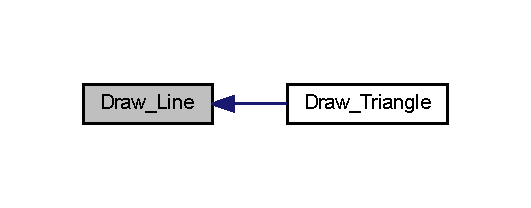
\includegraphics[width=255pt]{_draw__request_8h_a978257370e90e9832a47bb67a51bcdd0_icgraph}
\end{center}
\end{figure}
\mbox{\Hypertarget{_draw__request_8h_afcc60b34bed9039c997f6d923fb50e4c}\label{_draw__request_8h_afcc60b34bed9039c997f6d923fb50e4c}} 
\index{Draw\+\_\+request.\+h@{Draw\+\_\+request.\+h}!Draw\+\_\+\+Rectangle@{Draw\+\_\+\+Rectangle}}
\index{Draw\+\_\+\+Rectangle@{Draw\+\_\+\+Rectangle}!Draw\+\_\+request.\+h@{Draw\+\_\+request.\+h}}
\subsubsection{\texorpdfstring{Draw\+\_\+\+Rectangle()}{Draw\_Rectangle()}}
{\footnotesize\ttfamily void Draw\+\_\+\+Rectangle (\begin{DoxyParamCaption}\item[{uint16\+\_\+t}]{xp,  }\item[{uint16\+\_\+t}]{yp,  }\item[{uint8\+\_\+t}]{x\+\_\+length,  }\item[{uint8\+\_\+t}]{y\+\_\+length,  }\item[{uint8\+\_\+t}]{line\+\_\+width,  }\item[{uint8\+\_\+t}]{fill,  }\item[{uint8\+\_\+t}]{color }\end{DoxyParamCaption})}



Draws a rectangle with any lengths you like on a V\+GA screen. 


\begin{DoxyParams}{Parameters}
{\em xp} & x value of the start coordinate (0 to 320). \\
\hline
{\em yp} & y value of the start coordinate (0 to 240). \\
\hline
{\em x\+\_\+length} & the amount of pixels in the x direction (0 to 320 minus xp). \\
\hline
{\em y\+\_\+length} & the amount of pixels in the y direction (0 to 240 minus yp). \\
\hline
{\em line\+\_\+width} & the width of the drawn line (1 to half of the shortest length). \\
\hline
{\em fill} & filled rectangle (1) or empty rectangle (0). \\
\hline
{\em color} & color of the rectangle (0x00 to 0x\+FF). \\
\hline
\end{DoxyParams}
\begin{DoxyRemark}{Remarks}
{\bfseries Memory} 
\end{DoxyRemark}
\mbox{\Hypertarget{_draw__request_8h_ad403fe7bfee17d66ba92bdb7a8d13079}\label{_draw__request_8h_ad403fe7bfee17d66ba92bdb7a8d13079}} 
\index{Draw\+\_\+request.\+h@{Draw\+\_\+request.\+h}!draw\+\_\+sentence@{draw\+\_\+sentence}}
\index{draw\+\_\+sentence@{draw\+\_\+sentence}!Draw\+\_\+request.\+h@{Draw\+\_\+request.\+h}}
\subsubsection{\texorpdfstring{draw\+\_\+sentence()}{draw\_sentence()}}
{\footnotesize\ttfamily void draw\+\_\+sentence (\begin{DoxyParamCaption}\item[{uint16\+\_\+t}]{xp,  }\item[{uint16\+\_\+t}]{yp,  }\item[{char $\ast$}]{sent,  }\item[{uint8\+\_\+t}]{color,  }\item[{\hyperlink{_draw__request_8h_a5f885badaea1ce688c8349bc79e82358}{f\+\_\+name}}]{font\+\_\+name,  }\item[{\hyperlink{_draw__request_8h_afeee049c9120627f4bad4322d131c130}{f\+\_\+type}}]{font\+\_\+type,  }\item[{uint8\+\_\+t}]{font\+\_\+size,  }\item[{uint8\+\_\+t}]{bg }\end{DoxyParamCaption})}



Draw multiple characyers on the V\+GA screen. 


\begin{DoxyParams}{Parameters}
{\em xp} & x value of the pixel coordinate (0 to 320). \\
\hline
{\em yp} & y value of the pixel coordinate (0 to 240). \\
\hline
{\em color} & color of the pixel (0x00 to 0x\+FF). \\
\hline
{\em font\+\_\+name} & \\
\hline
{\em font\+\_\+type} & \\
\hline
{\em font\+\_\+size} & \\
\hline
{\em bg} & background color. \\
\hline
\end{DoxyParams}
\begin{DoxyRemark}{Remarks}
{\bfseries Memory} 

{\bfseries Milestone} 
\end{DoxyRemark}
\mbox{\Hypertarget{_draw__request_8h_a6d2f3b22c1ae88122730df5de2981cd7}\label{_draw__request_8h_a6d2f3b22c1ae88122730df5de2981cd7}} 
\index{Draw\+\_\+request.\+h@{Draw\+\_\+request.\+h}!Draw\+\_\+\+Triangle@{Draw\+\_\+\+Triangle}}
\index{Draw\+\_\+\+Triangle@{Draw\+\_\+\+Triangle}!Draw\+\_\+request.\+h@{Draw\+\_\+request.\+h}}
\subsubsection{\texorpdfstring{Draw\+\_\+\+Triangle()}{Draw\_Triangle()}}
{\footnotesize\ttfamily void Draw\+\_\+\+Triangle (\begin{DoxyParamCaption}\item[{uint16\+\_\+t}]{x1,  }\item[{uint16\+\_\+t}]{y1,  }\item[{uint16\+\_\+t}]{x2,  }\item[{uint16\+\_\+t}]{y2,  }\item[{uint16\+\_\+t}]{x3,  }\item[{uint16\+\_\+t}]{y3,  }\item[{int}]{fill,  }\item[{uint8\+\_\+t}]{line\+\_\+width,  }\item[{uint8\+\_\+t}]{color }\end{DoxyParamCaption})}



Draws a triangle with the corners on which ever coordinate you choose. 


\begin{DoxyParams}{Parameters}
{\em x1} & x value of the first coordinate (0 to 320). \\
\hline
{\em y1} & y value of the first coordinate (0 to 240). \\
\hline
{\em x2} & x value of the second coordinate (0 to 320). \\
\hline
{\em y2} & y value of the second coordinate (0 to 240). \\
\hline
{\em x3} & x value of the third coordinate (0 to 320). \\
\hline
{\em y3} & y value of the third coordinate (0 to 240). \\
\hline
{\em fill} & filled triangle (1) or empty triangle (0). \\
\hline
{\em color} & color of the triangle (0x00 to 0x\+FF). \\
\hline
\end{DoxyParams}
\begin{DoxyRemark}{Remarks}
{\bfseries Memory} 

{\bfseries Milestone} It could be faster without all the mathematical stuff going on. 
\end{DoxyRemark}
Here is the call graph for this function\+:\nopagebreak
\begin{figure}[H]
\begin{center}
\leavevmode
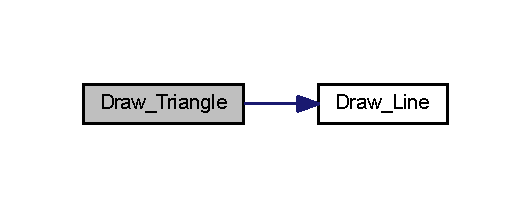
\includegraphics[width=255pt]{_draw__request_8h_a6d2f3b22c1ae88122730df5de2981cd7_cgraph}
\end{center}
\end{figure}
\mbox{\Hypertarget{_draw__request_8h_a1c72a0e7b90d716ea89145be3b2ac374}\label{_draw__request_8h_a1c72a0e7b90d716ea89145be3b2ac374}} 
\index{Draw\+\_\+request.\+h@{Draw\+\_\+request.\+h}!Draw\+\_\+\+Ver\+Line@{Draw\+\_\+\+Ver\+Line}}
\index{Draw\+\_\+\+Ver\+Line@{Draw\+\_\+\+Ver\+Line}!Draw\+\_\+request.\+h@{Draw\+\_\+request.\+h}}
\subsubsection{\texorpdfstring{Draw\+\_\+\+Ver\+Line()}{Draw\_VerLine()}}
{\footnotesize\ttfamily void Draw\+\_\+\+Ver\+Line (\begin{DoxyParamCaption}\item[{uint16\+\_\+t}]{xp,  }\item[{uint16\+\_\+t}]{yp,  }\item[{uint8\+\_\+t}]{length,  }\item[{uint8\+\_\+t}]{color }\end{DoxyParamCaption})}



Draws a vertical line on a V\+GA screen. 


\begin{DoxyParams}{Parameters}
{\em xp} & x value of the start coordinate (0 to 320). \\
\hline
{\em yp} & y value of the start coordinate (0 to 240). \\
\hline
{\em length} & amount of pixels that makes the length of the line. \\
\hline
{\em color} & color of the line (0x00 to 0x\+FF). \\
\hline
\end{DoxyParams}
\begin{DoxyRemark}{Remarks}
{\bfseries Memory} 
\end{DoxyRemark}
\mbox{\Hypertarget{_draw__request_8h_aadb59076e96776dbf24e0a6620de0400}\label{_draw__request_8h_aadb59076e96776dbf24e0a6620de0400}} 
\index{Draw\+\_\+request.\+h@{Draw\+\_\+request.\+h}!Set\+\_\+\+Single\+\_\+\+Pixel@{Set\+\_\+\+Single\+\_\+\+Pixel}}
\index{Set\+\_\+\+Single\+\_\+\+Pixel@{Set\+\_\+\+Single\+\_\+\+Pixel}!Draw\+\_\+request.\+h@{Draw\+\_\+request.\+h}}
\subsubsection{\texorpdfstring{Set\+\_\+\+Single\+\_\+\+Pixel()}{Set\_Single\_Pixel()}}
{\footnotesize\ttfamily void Set\+\_\+\+Single\+\_\+\+Pixel (\begin{DoxyParamCaption}\item[{uint16\+\_\+t}]{xp,  }\item[{uint16\+\_\+t}]{yp,  }\item[{uint8\+\_\+t}]{colour }\end{DoxyParamCaption})}



Colors a pixel on the coordinate of you desire with the color of your desire. 


\begin{DoxyParams}{Parameters}
{\em xp} & x value of the pixel coordinate (0 to 320). \\
\hline
{\em yp} & y value of the pixel coordinate (0 to 240). \\
\hline
{\em color} & color of the pixel (0x00 to 0x\+FF). \\
\hline
\end{DoxyParams}
\begin{DoxyRemark}{Remarks}
{\bfseries Memory} 

{\bfseries Milestone} 
\end{DoxyRemark}
\mbox{\Hypertarget{_draw__request_8h_ab72b41a355531a67fbecd509c90edde9}\label{_draw__request_8h_ab72b41a355531a67fbecd509c90edde9}} 
\index{Draw\+\_\+request.\+h@{Draw\+\_\+request.\+h}!T\+I\+M\+E\+R3\+\_\+\+Initialize@{T\+I\+M\+E\+R3\+\_\+\+Initialize}}
\index{T\+I\+M\+E\+R3\+\_\+\+Initialize@{T\+I\+M\+E\+R3\+\_\+\+Initialize}!Draw\+\_\+request.\+h@{Draw\+\_\+request.\+h}}
\subsubsection{\texorpdfstring{T\+I\+M\+E\+R3\+\_\+\+Initialize()}{TIMER3\_Initialize()}}
{\footnotesize\ttfamily void T\+I\+M\+E\+R3\+\_\+\+Initialize (\begin{DoxyParamCaption}{ }\end{DoxyParamCaption})}



Timer3 Initialization. 

Here is the caller graph for this function\+:\nopagebreak
\begin{figure}[H]
\begin{center}
\leavevmode
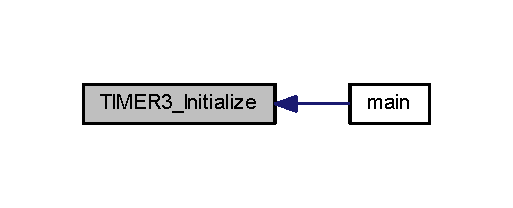
\includegraphics[width=246pt]{_draw__request_8h_ab72b41a355531a67fbecd509c90edde9_icgraph}
\end{center}
\end{figure}
\mbox{\Hypertarget{_draw__request_8h_a36c40ce15fec581ea1d076aea9a41b12}\label{_draw__request_8h_a36c40ce15fec581ea1d076aea9a41b12}} 
\index{Draw\+\_\+request.\+h@{Draw\+\_\+request.\+h}!wait\+\_\+msec@{wait\+\_\+msec}}
\index{wait\+\_\+msec@{wait\+\_\+msec}!Draw\+\_\+request.\+h@{Draw\+\_\+request.\+h}}
\subsubsection{\texorpdfstring{wait\+\_\+msec()}{wait\_msec()}}
{\footnotesize\ttfamily void wait\+\_\+msec (\begin{DoxyParamCaption}\item[{unsigned int}]{msec }\end{DoxyParamCaption})}


\begin{DoxyParams}{Parameters}
{\em msec} & \\
\hline
\end{DoxyParams}
\begin{DoxyRemark}{Remarks}
Memory\+: 

Wat kan er beter? 
\end{DoxyRemark}

\hypertarget{uitvoer_8h}{}\section{logic\+\_\+layer/uitvoer.h File Reference}
\label{uitvoer_8h}\index{logic\+\_\+layer/uitvoer.\+h@{logic\+\_\+layer/uitvoer.\+h}}
{\ttfamily \#include \char`\"{}stm32f4xx.\+h\char`\"{}}\newline
Include dependency graph for uitvoer.\+h\+:\nopagebreak
\begin{figure}[H]
\begin{center}
\leavevmode
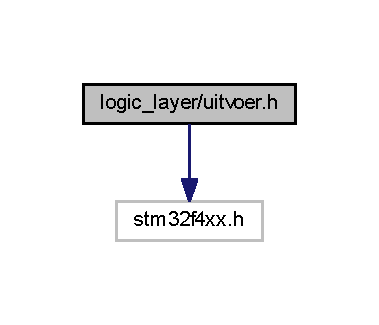
\includegraphics[width=182pt]{uitvoer_8h__incl}
\end{center}
\end{figure}
This graph shows which files directly or indirectly include this file\+:\nopagebreak
\begin{figure}[H]
\begin{center}
\leavevmode
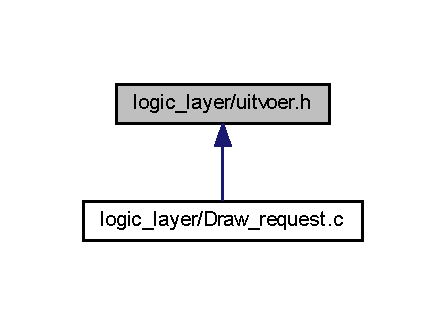
\includegraphics[width=214pt]{uitvoer_8h__dep__incl}
\end{center}
\end{figure}
\subsection*{Macros}
\begin{DoxyCompactItemize}
\item 
\#define \hyperlink{uitvoer_8h_aafd9a8a07447ca0c0c79ae00e8e5f7e9}{I\+M\+A\+G\+E\+\_\+\+W\+I\+D\+TH}~80
\item 
\#define \hyperlink{uitvoer_8h_a24688fc70fd5d6fe90a57e03a34ebc1c}{I\+M\+A\+G\+E\+\_\+\+H\+E\+I\+G\+HT}~60
\item 
\#define \hyperlink{uitvoer_8h_a6850a77c3bb678e4869349b455d685b4}{I\+M\+A\+G\+E\+\_\+\+T\+Y\+PE}~1
\end{DoxyCompactItemize}
\subsection*{Variables}
\begin{DoxyCompactItemize}
\item 
const uint8\+\_\+t \hyperlink{uitvoer_8h_a5d4fa827289174127b6a2db1bb83f52c}{pijl\+\_\+rechts} \mbox{[}$\,$\mbox{]}
\item 
const uint8\+\_\+t \hyperlink{uitvoer_8h_a98a7042ac9a526a07494719d38bd43c4}{pijl\+\_\+links} \mbox{[}$\,$\mbox{]}
\item 
const uint8\+\_\+t \hyperlink{uitvoer_8h_a304d09c81865532e704cd29958597cd5}{pijl\+\_\+omlaag} \mbox{[}$\,$\mbox{]}
\item 
const uint8\+\_\+t \hyperlink{uitvoer_8h_a9564ab3e08e274b4668db722bc837e1b}{pijl\+\_\+omhoog} \mbox{[}$\,$\mbox{]}
\item 
const uint8\+\_\+t \hyperlink{uitvoer_8h_a2c2b21491b539385241a507418ba9ba9}{smiley\+\_\+cool} \mbox{[}$\,$\mbox{]}
\item 
const uint8\+\_\+t \hyperlink{uitvoer_8h_a42f2a455ba6bc997a1de325dbe841c70}{smiley\+\_\+thumb} \mbox{[}$\,$\mbox{]}
\end{DoxyCompactItemize}


\subsection{Macro Definition Documentation}
\mbox{\Hypertarget{uitvoer_8h_a24688fc70fd5d6fe90a57e03a34ebc1c}\label{uitvoer_8h_a24688fc70fd5d6fe90a57e03a34ebc1c}} 
\index{uitvoer.\+h@{uitvoer.\+h}!I\+M\+A\+G\+E\+\_\+\+H\+E\+I\+G\+HT@{I\+M\+A\+G\+E\+\_\+\+H\+E\+I\+G\+HT}}
\index{I\+M\+A\+G\+E\+\_\+\+H\+E\+I\+G\+HT@{I\+M\+A\+G\+E\+\_\+\+H\+E\+I\+G\+HT}!uitvoer.\+h@{uitvoer.\+h}}
\subsubsection{\texorpdfstring{I\+M\+A\+G\+E\+\_\+\+H\+E\+I\+G\+HT}{IMAGE\_HEIGHT}}
{\footnotesize\ttfamily \#define I\+M\+A\+G\+E\+\_\+\+H\+E\+I\+G\+HT~60}

\mbox{\Hypertarget{uitvoer_8h_a6850a77c3bb678e4869349b455d685b4}\label{uitvoer_8h_a6850a77c3bb678e4869349b455d685b4}} 
\index{uitvoer.\+h@{uitvoer.\+h}!I\+M\+A\+G\+E\+\_\+\+T\+Y\+PE@{I\+M\+A\+G\+E\+\_\+\+T\+Y\+PE}}
\index{I\+M\+A\+G\+E\+\_\+\+T\+Y\+PE@{I\+M\+A\+G\+E\+\_\+\+T\+Y\+PE}!uitvoer.\+h@{uitvoer.\+h}}
\subsubsection{\texorpdfstring{I\+M\+A\+G\+E\+\_\+\+T\+Y\+PE}{IMAGE\_TYPE}}
{\footnotesize\ttfamily \#define I\+M\+A\+G\+E\+\_\+\+T\+Y\+PE~1}

\mbox{\Hypertarget{uitvoer_8h_aafd9a8a07447ca0c0c79ae00e8e5f7e9}\label{uitvoer_8h_aafd9a8a07447ca0c0c79ae00e8e5f7e9}} 
\index{uitvoer.\+h@{uitvoer.\+h}!I\+M\+A\+G\+E\+\_\+\+W\+I\+D\+TH@{I\+M\+A\+G\+E\+\_\+\+W\+I\+D\+TH}}
\index{I\+M\+A\+G\+E\+\_\+\+W\+I\+D\+TH@{I\+M\+A\+G\+E\+\_\+\+W\+I\+D\+TH}!uitvoer.\+h@{uitvoer.\+h}}
\subsubsection{\texorpdfstring{I\+M\+A\+G\+E\+\_\+\+W\+I\+D\+TH}{IMAGE\_WIDTH}}
{\footnotesize\ttfamily \#define I\+M\+A\+G\+E\+\_\+\+W\+I\+D\+TH~80}



\subsection{Variable Documentation}
\mbox{\Hypertarget{uitvoer_8h_a98a7042ac9a526a07494719d38bd43c4}\label{uitvoer_8h_a98a7042ac9a526a07494719d38bd43c4}} 
\index{uitvoer.\+h@{uitvoer.\+h}!pijl\+\_\+links@{pijl\+\_\+links}}
\index{pijl\+\_\+links@{pijl\+\_\+links}!uitvoer.\+h@{uitvoer.\+h}}
\subsubsection{\texorpdfstring{pijl\+\_\+links}{pijl\_links}}
{\footnotesize\ttfamily const uint8\+\_\+t pijl\+\_\+links\mbox{[}$\,$\mbox{]}}

\mbox{\Hypertarget{uitvoer_8h_a9564ab3e08e274b4668db722bc837e1b}\label{uitvoer_8h_a9564ab3e08e274b4668db722bc837e1b}} 
\index{uitvoer.\+h@{uitvoer.\+h}!pijl\+\_\+omhoog@{pijl\+\_\+omhoog}}
\index{pijl\+\_\+omhoog@{pijl\+\_\+omhoog}!uitvoer.\+h@{uitvoer.\+h}}
\subsubsection{\texorpdfstring{pijl\+\_\+omhoog}{pijl\_omhoog}}
{\footnotesize\ttfamily const uint8\+\_\+t pijl\+\_\+omhoog\mbox{[}$\,$\mbox{]}}

\mbox{\Hypertarget{uitvoer_8h_a304d09c81865532e704cd29958597cd5}\label{uitvoer_8h_a304d09c81865532e704cd29958597cd5}} 
\index{uitvoer.\+h@{uitvoer.\+h}!pijl\+\_\+omlaag@{pijl\+\_\+omlaag}}
\index{pijl\+\_\+omlaag@{pijl\+\_\+omlaag}!uitvoer.\+h@{uitvoer.\+h}}
\subsubsection{\texorpdfstring{pijl\+\_\+omlaag}{pijl\_omlaag}}
{\footnotesize\ttfamily const uint8\+\_\+t pijl\+\_\+omlaag\mbox{[}$\,$\mbox{]}}

\mbox{\Hypertarget{uitvoer_8h_a5d4fa827289174127b6a2db1bb83f52c}\label{uitvoer_8h_a5d4fa827289174127b6a2db1bb83f52c}} 
\index{uitvoer.\+h@{uitvoer.\+h}!pijl\+\_\+rechts@{pijl\+\_\+rechts}}
\index{pijl\+\_\+rechts@{pijl\+\_\+rechts}!uitvoer.\+h@{uitvoer.\+h}}
\subsubsection{\texorpdfstring{pijl\+\_\+rechts}{pijl\_rechts}}
{\footnotesize\ttfamily const uint8\+\_\+t pijl\+\_\+rechts\mbox{[}$\,$\mbox{]}}

\mbox{\Hypertarget{uitvoer_8h_a2c2b21491b539385241a507418ba9ba9}\label{uitvoer_8h_a2c2b21491b539385241a507418ba9ba9}} 
\index{uitvoer.\+h@{uitvoer.\+h}!smiley\+\_\+cool@{smiley\+\_\+cool}}
\index{smiley\+\_\+cool@{smiley\+\_\+cool}!uitvoer.\+h@{uitvoer.\+h}}
\subsubsection{\texorpdfstring{smiley\+\_\+cool}{smiley\_cool}}
{\footnotesize\ttfamily const uint8\+\_\+t smiley\+\_\+cool\mbox{[}$\,$\mbox{]}}

\mbox{\Hypertarget{uitvoer_8h_a42f2a455ba6bc997a1de325dbe841c70}\label{uitvoer_8h_a42f2a455ba6bc997a1de325dbe841c70}} 
\index{uitvoer.\+h@{uitvoer.\+h}!smiley\+\_\+thumb@{smiley\+\_\+thumb}}
\index{smiley\+\_\+thumb@{smiley\+\_\+thumb}!uitvoer.\+h@{uitvoer.\+h}}
\subsubsection{\texorpdfstring{smiley\+\_\+thumb}{smiley\_thumb}}
{\footnotesize\ttfamily const uint8\+\_\+t smiley\+\_\+thumb\mbox{[}$\,$\mbox{]}}


\hypertarget{main_8c}{}\section{main.\+c File Reference}
\label{main_8c}\index{main.\+c@{main.\+c}}
{\ttfamily \#include \char`\"{}includes.\+h\char`\"{}}\newline
{\ttfamily \#include \char`\"{}main.\+h\char`\"{}}\newline
Include dependency graph for main.\+c\+:\nopagebreak
\begin{figure}[H]
\begin{center}
\leavevmode
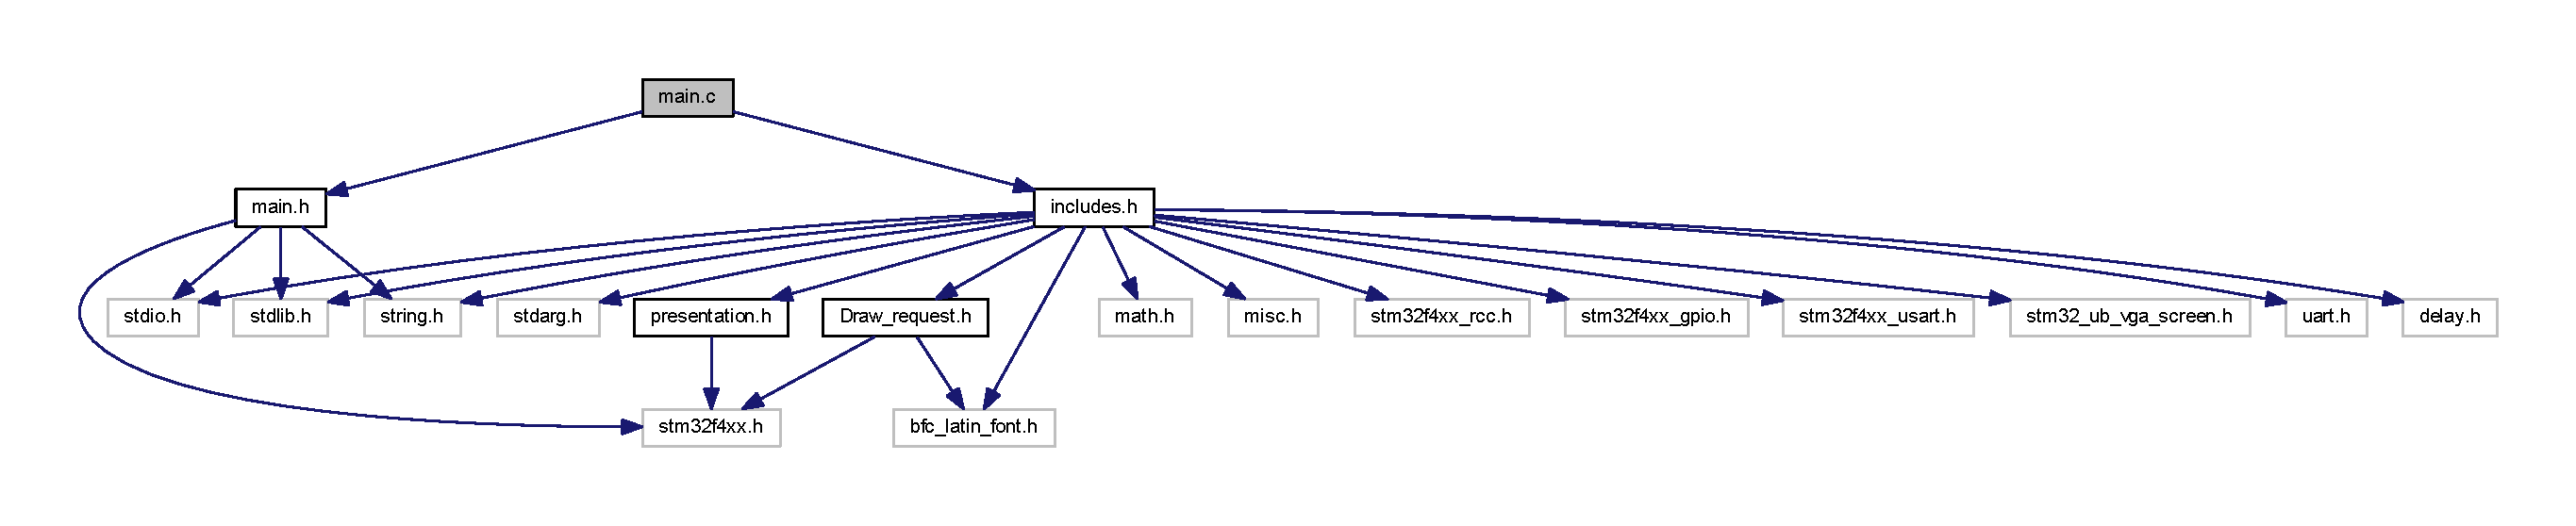
\includegraphics[width=350pt]{main_8c__incl}
\end{center}
\end{figure}
\subsection*{Functions}
\begin{DoxyCompactItemize}
\item 
int \hyperlink{main_8c_ae66f6b31b5ad750f1fe042a706a4e3d4}{main} ()
\end{DoxyCompactItemize}


\subsection{Function Documentation}
\mbox{\Hypertarget{main_8c_ae66f6b31b5ad750f1fe042a706a4e3d4}\label{main_8c_ae66f6b31b5ad750f1fe042a706a4e3d4}} 
\index{main.\+c@{main.\+c}!main@{main}}
\index{main@{main}!main.\+c@{main.\+c}}
\subsubsection{\texorpdfstring{main()}{main()}}
{\footnotesize\ttfamily int main (\begin{DoxyParamCaption}{ }\end{DoxyParamCaption})}

Here is the call graph for this function\+:\nopagebreak
\begin{figure}[H]
\begin{center}
\leavevmode
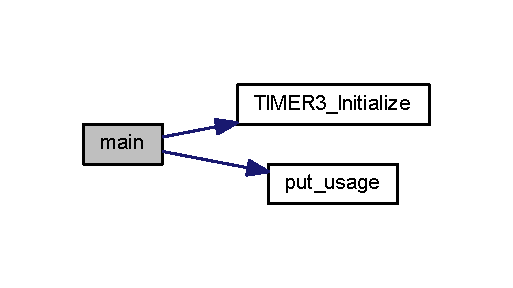
\includegraphics[width=246pt]{main_8c_ae66f6b31b5ad750f1fe042a706a4e3d4_cgraph}
\end{center}
\end{figure}

\hypertarget{main_8h}{}\section{main.\+h File Reference}
\label{main_8h}\index{main.\+h@{main.\+h}}
{\ttfamily \#include \char`\"{}stm32f4xx.\+h\char`\"{}}\newline
{\ttfamily \#include \char`\"{}stdio.\+h\char`\"{}}\newline
{\ttfamily \#include $<$stdlib.\+h$>$}\newline
{\ttfamily \#include $<$string.\+h$>$}\newline
Include dependency graph for main.\+h\+:\nopagebreak
\begin{figure}[H]
\begin{center}
\leavevmode
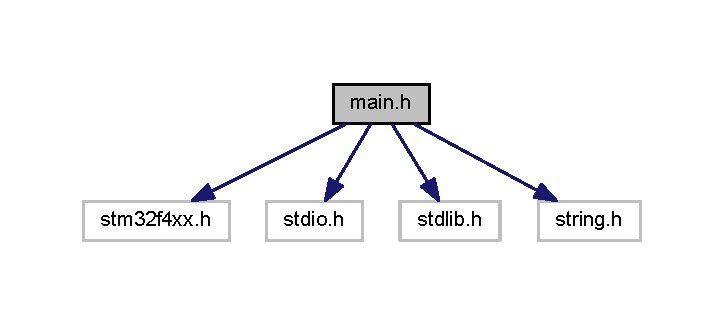
\includegraphics[width=348pt]{main_8h__incl}
\end{center}
\end{figure}
This graph shows which files directly or indirectly include this file\+:\nopagebreak
\begin{figure}[H]
\begin{center}
\leavevmode
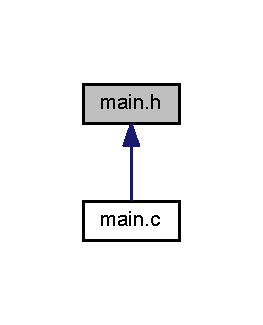
\includegraphics[width=126pt]{main_8h__dep__incl}
\end{center}
\end{figure}

\hypertarget{presentation_8c}{}\section{Presentation\+\_\+layer/presentation.c File Reference}
\label{presentation_8c}\index{Presentation\+\_\+layer/presentation.\+c@{Presentation\+\_\+layer/presentation.\+c}}
{\ttfamily \#include \char`\"{}includes.\+h\char`\"{}}\newline
Include dependency graph for presentation.\+c\+:\nopagebreak
\begin{figure}[H]
\begin{center}
\leavevmode
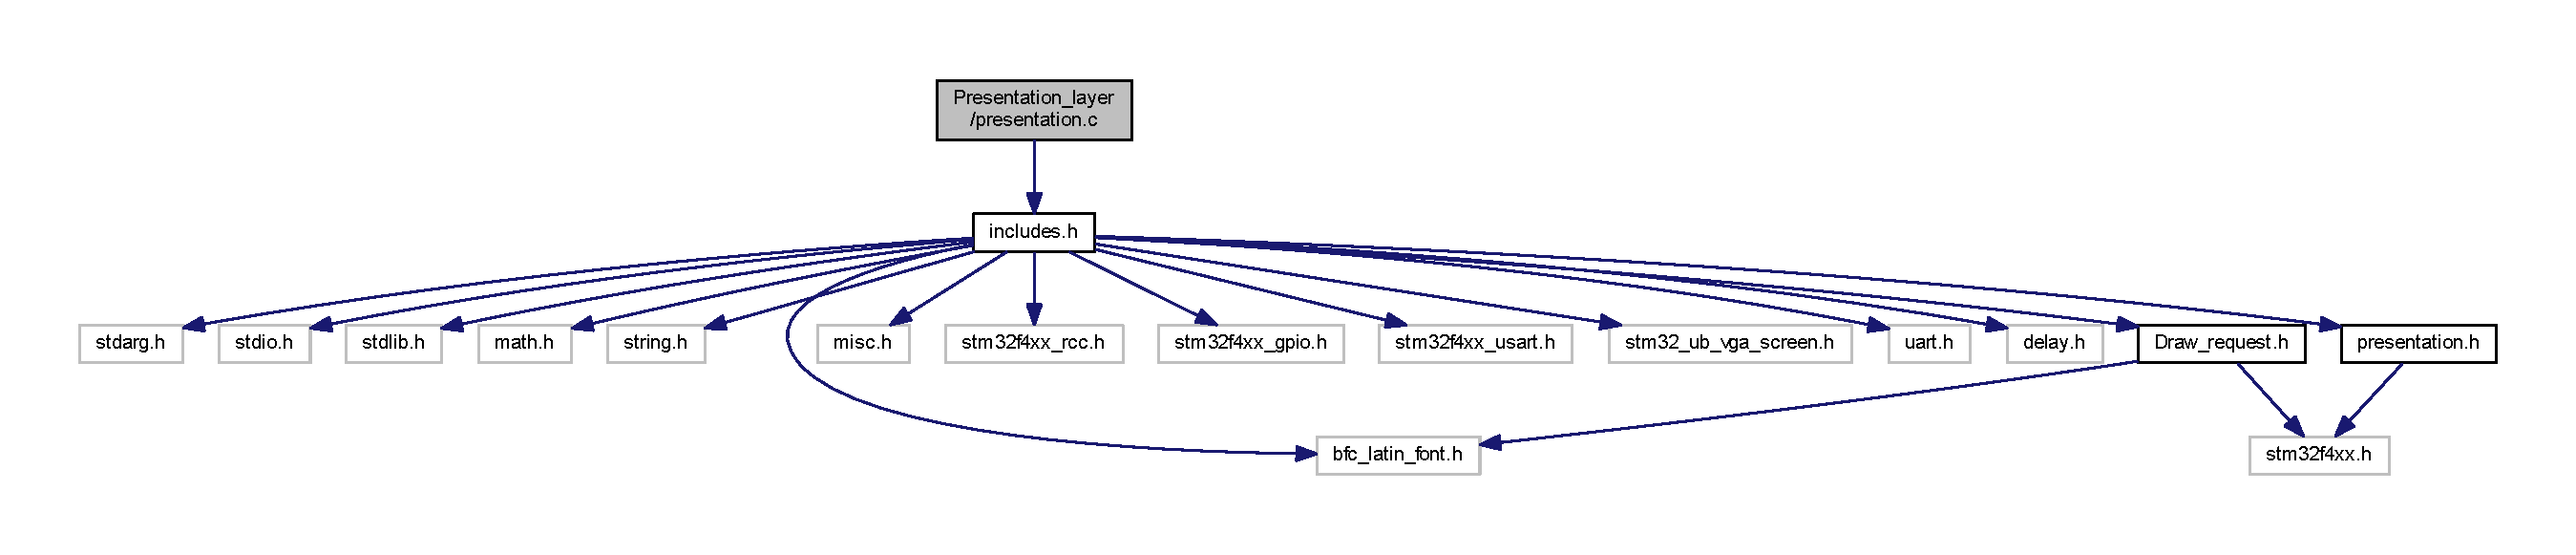
\includegraphics[width=350pt]{presentation_8c__incl}
\end{center}
\end{figure}
\subsection*{Functions}
\begin{DoxyCompactItemize}
\item 
int \hyperlink{presentation_8c_a9bcf610e4b03d34b8e4f287006a54df7}{line\+\_\+split} (char $\ast$str, char separator, char $\ast$$\ast$$\ast$array, int $\ast$length)
\item 
void \hyperlink{presentation_8c_a772b49869c6e14a71075467d854ef8a7}{put\+\_\+usage} ()
\begin{DoxyCompactList}\small\item\em The instructions of how you should use the software with the terminal, to be printed in the terminal. \end{DoxyCompactList}\item 
void \hyperlink{presentation_8c_a1ea3d6e2ebf24a088e98b93b870ef1ef}{Request\+\_\+\+Handling} (char $\ast$$\ast$res)
\end{DoxyCompactItemize}


\subsection{Function Documentation}
\mbox{\Hypertarget{presentation_8c_a9bcf610e4b03d34b8e4f287006a54df7}\label{presentation_8c_a9bcf610e4b03d34b8e4f287006a54df7}} 
\index{presentation.\+c@{presentation.\+c}!line\+\_\+split@{line\+\_\+split}}
\index{line\+\_\+split@{line\+\_\+split}!presentation.\+c@{presentation.\+c}}
\subsubsection{\texorpdfstring{line\+\_\+split()}{line\_split()}}
{\footnotesize\ttfamily int line\+\_\+split (\begin{DoxyParamCaption}\item[{char $\ast$}]{str,  }\item[{char}]{separator,  }\item[{char $\ast$$\ast$$\ast$}]{array,  }\item[{int $\ast$}]{length }\end{DoxyParamCaption})}






\begin{DoxyParams}{Parameters}
{\em $\ast$str} & \\
\hline
{\em separator} & \\
\hline
{\em $\ast$$\ast$$\ast$array} & \\
\hline
{\em $\ast$length} & \\
\hline
\end{DoxyParams}
\begin{DoxyReturn}{Returns}
0 
\end{DoxyReturn}
\begin{DoxyRemark}{Remarks}
{\bfseries Memory} 

{\bfseries Milestone} 
\end{DoxyRemark}
\mbox{\Hypertarget{presentation_8c_a772b49869c6e14a71075467d854ef8a7}\label{presentation_8c_a772b49869c6e14a71075467d854ef8a7}} 
\index{presentation.\+c@{presentation.\+c}!put\+\_\+usage@{put\+\_\+usage}}
\index{put\+\_\+usage@{put\+\_\+usage}!presentation.\+c@{presentation.\+c}}
\subsubsection{\texorpdfstring{put\+\_\+usage()}{put\_usage()}}
{\footnotesize\ttfamily void put\+\_\+usage (\begin{DoxyParamCaption}{ }\end{DoxyParamCaption})}



The instructions of how you should use the software with the terminal, to be printed in the terminal. 


\begin{DoxyParams}{Parameters}
{\em $\ast$$\ast$res} & \\
\hline
\end{DoxyParams}
\begin{DoxyRemark}{Remarks}
{\bfseries Memory} 

{\bfseries Milestone} 
\end{DoxyRemark}
Here is the caller graph for this function\+:\nopagebreak
\begin{figure}[H]
\begin{center}
\leavevmode
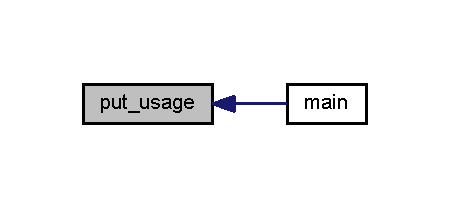
\includegraphics[width=216pt]{presentation_8c_a772b49869c6e14a71075467d854ef8a7_icgraph}
\end{center}
\end{figure}
\mbox{\Hypertarget{presentation_8c_a1ea3d6e2ebf24a088e98b93b870ef1ef}\label{presentation_8c_a1ea3d6e2ebf24a088e98b93b870ef1ef}} 
\index{presentation.\+c@{presentation.\+c}!Request\+\_\+\+Handling@{Request\+\_\+\+Handling}}
\index{Request\+\_\+\+Handling@{Request\+\_\+\+Handling}!presentation.\+c@{presentation.\+c}}
\subsubsection{\texorpdfstring{Request\+\_\+\+Handling()}{Request\_Handling()}}
{\footnotesize\ttfamily void Request\+\_\+\+Handling (\begin{DoxyParamCaption}\item[{char $\ast$$\ast$}]{res }\end{DoxyParamCaption})}






\begin{DoxyParams}{Parameters}
{\em $\ast$$\ast$res} & \\
\hline
\end{DoxyParams}
\begin{DoxyRemark}{Remarks}
{\bfseries Memory} 

{\bfseries Milestone} 
\end{DoxyRemark}

\hypertarget{presentation_8h}{}\section{Presentation\+\_\+layer/presentation.h File Reference}
\label{presentation_8h}\index{Presentation\+\_\+layer/presentation.\+h@{Presentation\+\_\+layer/presentation.\+h}}
{\ttfamily \#include \char`\"{}stm32f4xx.\+h\char`\"{}}\newline
Include dependency graph for presentation.\+h\+:\nopagebreak
\begin{figure}[H]
\begin{center}
\leavevmode
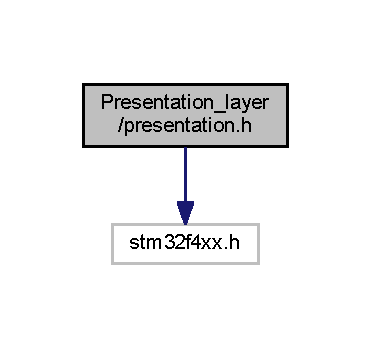
\includegraphics[width=178pt]{presentation_8h__incl}
\end{center}
\end{figure}
This graph shows which files directly or indirectly include this file\+:\nopagebreak
\begin{figure}[H]
\begin{center}
\leavevmode
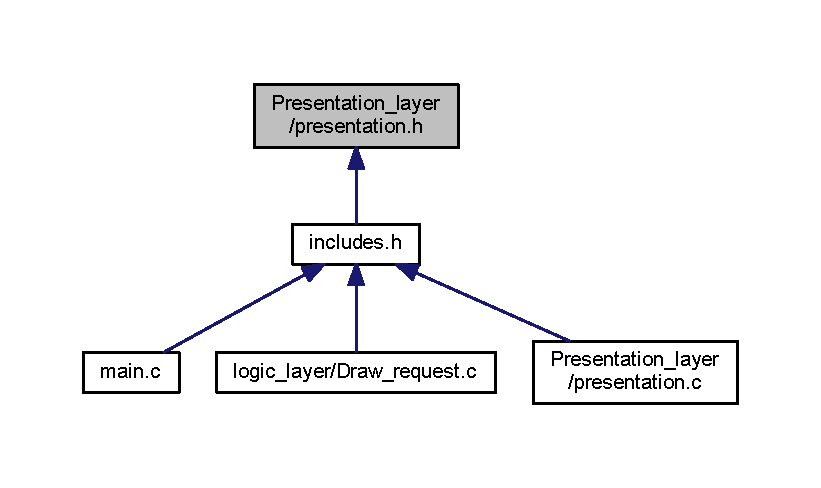
\includegraphics[width=350pt]{presentation_8h__dep__incl}
\end{center}
\end{figure}
\subsection*{Enumerations}
\begin{DoxyCompactItemize}
\item 
enum \hyperlink{presentation_8h_a51e6a0d2bcb8531a5e5adcd66a77aa3b}{request} \{ \newline
\hyperlink{presentation_8h_a51e6a0d2bcb8531a5e5adcd66a77aa3babbd80f5b3aeae14bc5c8039d1b98b8d3}{tekst}, 
\hyperlink{presentation_8h_a51e6a0d2bcb8531a5e5adcd66a77aa3ba0fbae7997a439c600969aa1ebf031f4f}{ellips}, 
\hyperlink{presentation_8h_a51e6a0d2bcb8531a5e5adcd66a77aa3ba5308a7a69e38caca569a2a6d9772b81e}{rechthoek}, 
\hyperlink{presentation_8h_a51e6a0d2bcb8531a5e5adcd66a77aa3ba83421c3afc5b98ba136ea22719102c5d}{driehoek}, 
\newline
\hyperlink{presentation_8h_a51e6a0d2bcb8531a5e5adcd66a77aa3badebc56589936fde95feb5e5e36d69edd}{lijn}, 
\hyperlink{presentation_8h_a51e6a0d2bcb8531a5e5adcd66a77aa3baa4c33f36ed157a7afdcb014a10e42d4b}{wacht}, 
\hyperlink{presentation_8h_a51e6a0d2bcb8531a5e5adcd66a77aa3ba998253d40e4c3cf2725ca6121cc904e4}{bitmap}
 \}
\end{DoxyCompactItemize}
\subsection*{Functions}
\begin{DoxyCompactItemize}
\item 
int \hyperlink{presentation_8h_a9bcf610e4b03d34b8e4f287006a54df7}{line\+\_\+split} (char $\ast$str, char separator, char $\ast$$\ast$$\ast$array, int $\ast$length)
\item 
void \hyperlink{presentation_8h_a1ea3d6e2ebf24a088e98b93b870ef1ef}{Request\+\_\+\+Handling} (char $\ast$$\ast$res)
\item 
void \hyperlink{presentation_8h_a772b49869c6e14a71075467d854ef8a7}{put\+\_\+usage} ()
\begin{DoxyCompactList}\small\item\em The instructions of how you should use the software with the terminal, to be printed in the terminal. \end{DoxyCompactList}\end{DoxyCompactItemize}


\subsection{Enumeration Type Documentation}
\mbox{\Hypertarget{presentation_8h_a51e6a0d2bcb8531a5e5adcd66a77aa3b}\label{presentation_8h_a51e6a0d2bcb8531a5e5adcd66a77aa3b}} 
\index{presentation.\+h@{presentation.\+h}!request@{request}}
\index{request@{request}!presentation.\+h@{presentation.\+h}}
\subsubsection{\texorpdfstring{request}{request}}
{\footnotesize\ttfamily enum \hyperlink{presentation_8h_a51e6a0d2bcb8531a5e5adcd66a77aa3b}{request}}

\begin{DoxyEnumFields}{Enumerator}
\raisebox{\heightof{T}}[0pt][0pt]{\index{tekst@{tekst}!presentation.\+h@{presentation.\+h}}\index{presentation.\+h@{presentation.\+h}!tekst@{tekst}}}\mbox{\Hypertarget{presentation_8h_a51e6a0d2bcb8531a5e5adcd66a77aa3babbd80f5b3aeae14bc5c8039d1b98b8d3}\label{presentation_8h_a51e6a0d2bcb8531a5e5adcd66a77aa3babbd80f5b3aeae14bc5c8039d1b98b8d3}} 
tekst&\\
\hline

\raisebox{\heightof{T}}[0pt][0pt]{\index{ellips@{ellips}!presentation.\+h@{presentation.\+h}}\index{presentation.\+h@{presentation.\+h}!ellips@{ellips}}}\mbox{\Hypertarget{presentation_8h_a51e6a0d2bcb8531a5e5adcd66a77aa3ba0fbae7997a439c600969aa1ebf031f4f}\label{presentation_8h_a51e6a0d2bcb8531a5e5adcd66a77aa3ba0fbae7997a439c600969aa1ebf031f4f}} 
ellips&\\
\hline

\raisebox{\heightof{T}}[0pt][0pt]{\index{rechthoek@{rechthoek}!presentation.\+h@{presentation.\+h}}\index{presentation.\+h@{presentation.\+h}!rechthoek@{rechthoek}}}\mbox{\Hypertarget{presentation_8h_a51e6a0d2bcb8531a5e5adcd66a77aa3ba5308a7a69e38caca569a2a6d9772b81e}\label{presentation_8h_a51e6a0d2bcb8531a5e5adcd66a77aa3ba5308a7a69e38caca569a2a6d9772b81e}} 
rechthoek&\\
\hline

\raisebox{\heightof{T}}[0pt][0pt]{\index{driehoek@{driehoek}!presentation.\+h@{presentation.\+h}}\index{presentation.\+h@{presentation.\+h}!driehoek@{driehoek}}}\mbox{\Hypertarget{presentation_8h_a51e6a0d2bcb8531a5e5adcd66a77aa3ba83421c3afc5b98ba136ea22719102c5d}\label{presentation_8h_a51e6a0d2bcb8531a5e5adcd66a77aa3ba83421c3afc5b98ba136ea22719102c5d}} 
driehoek&\\
\hline

\raisebox{\heightof{T}}[0pt][0pt]{\index{lijn@{lijn}!presentation.\+h@{presentation.\+h}}\index{presentation.\+h@{presentation.\+h}!lijn@{lijn}}}\mbox{\Hypertarget{presentation_8h_a51e6a0d2bcb8531a5e5adcd66a77aa3badebc56589936fde95feb5e5e36d69edd}\label{presentation_8h_a51e6a0d2bcb8531a5e5adcd66a77aa3badebc56589936fde95feb5e5e36d69edd}} 
lijn&\\
\hline

\raisebox{\heightof{T}}[0pt][0pt]{\index{wacht@{wacht}!presentation.\+h@{presentation.\+h}}\index{presentation.\+h@{presentation.\+h}!wacht@{wacht}}}\mbox{\Hypertarget{presentation_8h_a51e6a0d2bcb8531a5e5adcd66a77aa3baa4c33f36ed157a7afdcb014a10e42d4b}\label{presentation_8h_a51e6a0d2bcb8531a5e5adcd66a77aa3baa4c33f36ed157a7afdcb014a10e42d4b}} 
wacht&\\
\hline

\raisebox{\heightof{T}}[0pt][0pt]{\index{bitmap@{bitmap}!presentation.\+h@{presentation.\+h}}\index{presentation.\+h@{presentation.\+h}!bitmap@{bitmap}}}\mbox{\Hypertarget{presentation_8h_a51e6a0d2bcb8531a5e5adcd66a77aa3ba998253d40e4c3cf2725ca6121cc904e4}\label{presentation_8h_a51e6a0d2bcb8531a5e5adcd66a77aa3ba998253d40e4c3cf2725ca6121cc904e4}} 
bitmap&\\
\hline

\end{DoxyEnumFields}


\subsection{Function Documentation}
\mbox{\Hypertarget{presentation_8h_a9bcf610e4b03d34b8e4f287006a54df7}\label{presentation_8h_a9bcf610e4b03d34b8e4f287006a54df7}} 
\index{presentation.\+h@{presentation.\+h}!line\+\_\+split@{line\+\_\+split}}
\index{line\+\_\+split@{line\+\_\+split}!presentation.\+h@{presentation.\+h}}
\subsubsection{\texorpdfstring{line\+\_\+split()}{line\_split()}}
{\footnotesize\ttfamily int line\+\_\+split (\begin{DoxyParamCaption}\item[{char $\ast$}]{str,  }\item[{char}]{separator,  }\item[{char $\ast$$\ast$$\ast$}]{array,  }\item[{int $\ast$}]{length }\end{DoxyParamCaption})}






\begin{DoxyParams}{Parameters}
{\em $\ast$str} & \\
\hline
{\em separator} & \\
\hline
{\em $\ast$$\ast$$\ast$array} & \\
\hline
{\em $\ast$length} & \\
\hline
\end{DoxyParams}
\begin{DoxyReturn}{Returns}
0 
\end{DoxyReturn}
\begin{DoxyRemark}{Remarks}
{\bfseries Memory} 

{\bfseries Milestone} 
\end{DoxyRemark}
\mbox{\Hypertarget{presentation_8h_a772b49869c6e14a71075467d854ef8a7}\label{presentation_8h_a772b49869c6e14a71075467d854ef8a7}} 
\index{presentation.\+h@{presentation.\+h}!put\+\_\+usage@{put\+\_\+usage}}
\index{put\+\_\+usage@{put\+\_\+usage}!presentation.\+h@{presentation.\+h}}
\subsubsection{\texorpdfstring{put\+\_\+usage()}{put\_usage()}}
{\footnotesize\ttfamily void put\+\_\+usage (\begin{DoxyParamCaption}{ }\end{DoxyParamCaption})}



The instructions of how you should use the software with the terminal, to be printed in the terminal. 


\begin{DoxyParams}{Parameters}
{\em $\ast$$\ast$res} & \\
\hline
\end{DoxyParams}
\begin{DoxyRemark}{Remarks}
{\bfseries Memory} 

{\bfseries Milestone} 
\end{DoxyRemark}
Here is the caller graph for this function\+:\nopagebreak
\begin{figure}[H]
\begin{center}
\leavevmode
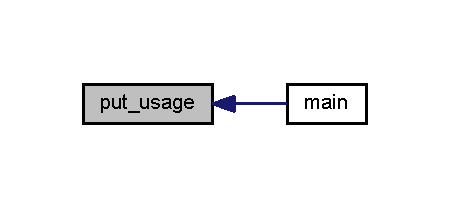
\includegraphics[width=216pt]{presentation_8h_a772b49869c6e14a71075467d854ef8a7_icgraph}
\end{center}
\end{figure}
\mbox{\Hypertarget{presentation_8h_a1ea3d6e2ebf24a088e98b93b870ef1ef}\label{presentation_8h_a1ea3d6e2ebf24a088e98b93b870ef1ef}} 
\index{presentation.\+h@{presentation.\+h}!Request\+\_\+\+Handling@{Request\+\_\+\+Handling}}
\index{Request\+\_\+\+Handling@{Request\+\_\+\+Handling}!presentation.\+h@{presentation.\+h}}
\subsubsection{\texorpdfstring{Request\+\_\+\+Handling()}{Request\_Handling()}}
{\footnotesize\ttfamily void Request\+\_\+\+Handling (\begin{DoxyParamCaption}\item[{char $\ast$$\ast$}]{res }\end{DoxyParamCaption})}






\begin{DoxyParams}{Parameters}
{\em $\ast$$\ast$res} & \\
\hline
\end{DoxyParams}
\begin{DoxyRemark}{Remarks}
{\bfseries Memory} 

{\bfseries Milestone} 
\end{DoxyRemark}

%--- End generated contents ---

% Index
\backmatter
\newpage
\phantomsection
\clearemptydoublepage
\addcontentsline{toc}{chapter}{Index}
\printindex

\end{document}
